\documentclass[a4paper,twoside,12pt]{article}

%% Page layout
\usepackage[margin=1in, headheight=16pt]{geometry}
\setlength{\marginparwidth}{2cm}

%% Metadata
\title{Multi-Fidelity Bayesian Optimisation of Ahmed Body Aerodynamics}
\author{Andrew Coyle}
\newcommand{\keywords}{Ahmed body, multi-fidelity, co-Kriging, Bayesian optimisation, DES, RANS, OpenFOAM, expected improvement}

%% Language and font
\usepackage[T1]{fontenc}
\usepackage[english]{babel}
\usepackage{mathpazo}
\usepackage{soul}

%% Units
\usepackage[squaren]{SIunits}

%% Bibliography
\usepackage[numbers]{natbib}

%% Paragraphs and spacing
\usepackage[parfill]{parskip}
\usepackage{setspace}
\onehalfspacing
\usepackage{enumitem}

%% Math
\usepackage{amsmath}
\usepackage{amssymb}

%% Quotes
\usepackage[autostyle=true]{csquotes}

%% Graphics and floats
\usepackage{graphicx}
\usepackage{float}
\usepackage{caption}
\usepackage{subcaption}
\captionsetup{font=small, labelfont=bf}
\usepackage{tikz}
\usetikzlibrary{arrows.meta, positioning, shapes.geometric}
\usepackage{pgfplots}
\pgfplotsset{compat=1.18}
\providecommand{\mathdefault}[1]{#1}

%% Tables
\usepackage{tabularx,booktabs}
\newcolumntype{C}{>{\centering\arraybackslash}X}
\usepackage{tablefootnote}

%% Links and metadata
\usepackage[colorlinks=true, allcolors=black]{hyperref}
\usepackage{hyperxmp}

%% Section formatting
\usepackage[compact]{titlesec}
\definecolor{accent_colour}{RGB}{5, 105, 185}

\usepackage{titling}
    \pretitle{\begin{center}\Large\bfseries\color{accent_colour}}
    \posttitle{\end{center}}
    \preauthor{\begin{center}\normalsize}
    \postauthor{\end{center}}
    \predate{\begin{center}\small}
    \postdate{\end{center}}
\titleformat{\section}{\normalfont\large\bfseries\color{accent_colour}}{\thesection}{10pt}{\large}[\titlerule]
\titlespacing*{\section}{0pt}{20pt}{20pt}
\titleformat{\subsection}{\normalfont\bfseries}{\thesubsection}{10pt}{}
\titlespacing*{\subsection}{0pt}{10pt}{10pt}

%% Headers/footers
\usepackage{fancyhdr}

\makeatletter
\hypersetup{
    pdftitle={\@title},
    pdfauthor={\@author},
    pdfkeywords={\keywords},
}
\makeatother

\begin{document}

\maketitle

\section*{Abstract}

A multi-fidelity Bayesian optimisation framework is applied to Ahmed body aerodynamics, minimising the objective $f_1 = C_d + \tfrac{1}{3}C_l$ (drag plus one-third downforce) over two geometric design variables: rear slant angle ($15$--$40^\circ$) and underbody diffuser angle ($0$--$20^\circ$). Low-fidelity evaluations use steady RANS (simpleFoam, $k$-$\omega$~SST) on the L2 mesh (${\sim}436$K half-domain cells, ${\sim}200$~s/solve); high-fidelity evaluations use the same solver on the L3 mesh (${\sim}912$K cells, ${\sim}500$~s/solve). A 30-point Phase~1 Latin Hypercube DoE screens four variables; Sobol sensitivity analysis eliminates nose radius and fixes ride height, reducing the active space to two dimensions. A 50-point Phase~2 DoE and 20 Bayesian optimisation iterations (Expected Improvement acquisition) identify the L2 surrogate optimum at $\alpha_\mathrm{slant}=32.5^\circ$, $\alpha_\mathrm{diff}=8.9^\circ$, $f_1=0.210$.

An L3 validation run at this point reveals a $\Delta C_l=+0.160$ fidelity gap (18\% objective degradation), motivating a Kennedy \& O'Hagan additive co-Kriging correction. Eight L3 anchor simulations spanning the full design space train correction Gaussian Processes $\delta_{C_d}(\mathbf{x})$ and $\delta_{C_l}(\mathbf{x})$. The corrections are spatially non-uniform ($\delta_{C_l}$ ranges $-0.114$ to $+0.167$), confirming that a constant bias correction would mis-locate the high-fidelity minimum. The corrected surrogate is re-optimised and the result verified with a single L3 solve.

The verified multi-fidelity optimum is $\alpha_\mathrm{slant}=38.9^\circ$, $\alpha_\mathrm{diff}=10.5^\circ$, $C_d=0.292$, $C_l=-0.285$, $f_1=0.198$ — a 5.7\% improvement over the L2 optimum and 20.2\% improvement over L3 evaluated at the old optimum location. Surrogate prediction error at the verified point is $0.6\%$, within the predicted $\pm2\sigma_\mathrm{HF}$ band. A $\lambda$-sensitivity sweep confirms the optimum location is robust for any positive downforce weighting. Basin-mapping L3 stencil solves confirm the optimum sits in a smooth basin, and resolve an anomalous L2 training point (BO iter~1, $f=0.642$) as a pseudo-time limit-cycle artefact that vanishes on the finer mesh. Total campaign cost: ${\sim}60$ CPU-hours.

\section{Introduction}
\label{sec:introduction}

Aerodynamic shape optimisation in motorsport requires navigating high-dimensional design spaces with expensive, high-fidelity simulations. Two competing concerns define the computational challenge: RANS closures are fast but systematically mis-predict separated flows, while scale-resolving methods (LES, DES) resolve those flows accurately but at orders-of-magnitude greater cost. Multi-fidelity surrogate modelling offers a principled path between them: a cheap low-fidelity model covers the design space densely, and expensive high-fidelity runs are used sparingly to correct the surrogate where fidelity matters most.

This report applies that framework to the \emph{Ahmed body} \cite{ahmed1984}, a canonical bluff body used throughout experimental and computational aerodynamics as a benchmark for road-vehicle rear-end flows. The geometry captures the two dominant aerodynamic phenomena relevant to motorsport ground vehicles: slant-induced flow separation and underbody ground effect. Its parametric simplicity---four independent design variables govern the rear aerodynamic character---makes it tractable for a full multi-fidelity campaign within a constrained compute budget.

\subsection{The Ahmed Body and Its Design Space}

The Ahmed body (Figure~\ref{fig:ahmed_schematic}) is a bluff body of length $L = 1044$~mm, width $W = 389$~mm, and height $H = 288$~mm, supported on four cylindrical feet. The rear of the body terminates in a slanted surface whose angle $\theta_s$ governs the dominant flow regime. Below a critical angle of approximately $30^\circ$, two counter-rotating longitudinal vortices originate at the slant edges and maintain partially attached flow across the slant; above $30^\circ$ the vortex system breaks down and the slant flow fully separates, paradoxically \emph{reducing} drag relative to the near-critical configuration \cite{lienhart2002}. The critical-angle regime has been extensively validated in wind-tunnel experiments at $\mathrm{Re}\approx2\times10^6$ and provides a natural benchmark for turbulence models.

Beyond the slant angle, three additional parameters are varied in this campaign. The underbody diffuser angle $\theta_d$ controls the rate of flow expansion beneath the rear of the body and directly sets the ground-effect downforce. The ride height $h$ sets the clearance between the body and the ground plane, governing the throat velocity and the magnitude of the suction pressure under the diffuser. The nose fillet radius $R_\mathrm{nose}$ modifies the front stagnation region and the leading-edge separation bubble; its aerodynamic impact is expected to be secondary but is included to prevent an artificially constrained design space.

The four-dimensional parameter bounds are:

\begin{table}[h]
    \centering
    \caption{Design variable bounds for the optimisation campaign.}
    \label{tab:design_variables}
    \begin{tabular}{lccl}
        \toprule
        Variable & Lower & Upper & Physical motivation \\
        \midrule
        Slant angle $\theta_s$ (deg) & 15 & 40 & Spans both sides of critical angle \\
        Diffuser angle $\theta_d$ (deg) & 0 & 20 & From flat underbody to strong diffuser \\
        Ride height $h$ (mm) & 30 & 80 & Ground clearance range \\
        Nose radius $R_\mathrm{nose}$ (mm) & 50 & 150 & Leading-edge separation sensitivity \\
        \bottomrule
    \end{tabular}
\end{table}

\subsection{Multi-Fidelity Co-Kriging}

The Kennedy \& O'Hagan (2000) co-Kriging model \cite{kennedy2000} decomposes the high-fidelity response as:

\begin{equation}
    f_\mathrm{HF}(\mathbf{x}) = f_\mathrm{LF}(\mathbf{x}) + \delta(\mathbf{x})
    \label{eq:cokriging}
\end{equation}

where $f_\mathrm{LF}$ is the RANS-trained Gaussian Process (GP) and $\delta(\mathbf{x})$ is an independent GP trained on the fidelity correction $f_\mathrm{HF} - f_\mathrm{LF}$ at the high-fidelity anchor simulation points. This additive formulation allows the correction GP to learn regions where the low-fidelity model is systematically wrong, without requiring any modification to the underlying RANS workflows at either fidelity level. Both GPs use a Mat\'{e}rn-$5/2$ kernel with automatic relevance determination (ARD), enabling the surrogate to identify the relative sensitivity of each design dimension.

\subsection{Bayesian Optimisation}

Bayesian Optimisation (BO) uses the co-Kriging surrogate's predictive mean and uncertainty to select the next most informative evaluation point via the Expected Improvement (EI) acquisition function \cite{jones1998}:

\begin{equation}
    \mathrm{EI}(\mathbf{x}) = \mathbb{E}\!\left[\max(f^* - f_\mathrm{HF}(\mathbf{x}),\, 0)\right]
    \label{eq:ei}
\end{equation}

where $f^*$ is the current best observed value of the aerodynamic efficiency objective. The EI quantifies the expected improvement over the current optimum, balancing exploration (high surrogate uncertainty) against exploitation (low surrogate mean). As the surrogate is refined with each new evaluation, EI should decay monotonically; convergence is declared when EI falls below a threshold.

\subsection{Objective Function}

The aerodynamic efficiency objective combines drag and downforce:

\begin{equation}
    f_1(\mathbf{x}) = C_d(\mathbf{x}) + \lambda\,C_l(\mathbf{x}), \qquad \lambda = \tfrac{1}{3}
    \label{eq:objective}
\end{equation}

where the sign convention is $C_l < 0$ for downforce and $C_l > 0$ for lift, and $\lambda = 1/3$ weights downforce three times less than drag in lap time terms. Minimising $f_1$ simultaneously pushes for low drag and negative $C_l$ (downforce); a reduction $\Delta C_l = -0.3$ is worth as much as $\Delta C_d = +0.1$ extra drag at this trade-off ratio.

\section{Methodology}
\label{sec:methodology}

\begin{figure}[h]
\centering
\begin{tikzpicture}[
    >=latex,
    every node/.style={font=\small},
    box/.style={draw=gray!55, rounded corners=3pt, fill=gray!8,
                minimum width=2.0cm, minimum height=0.65cm,
                align=center, inner sep=4pt},
    hibox/.style={draw=accent_colour!70, rounded corners=3pt, fill=accent_colour!10,
                minimum width=2.0cm, minimum height=0.65cm,
                align=center, inner sep=4pt},
    arr/.style={->, thick, gray!55!black},
    lbl/.style={font=\footnotesize, gray!55!black},
]
\node[box]   (doe)   at (0,   0) {RANS DoE\\(30 LHS pts)};
\node[box]   (des0)  at (3.0, 0) {DES anchors\\(10 pts)};
\node[hibox] (cok)   at (6.0, 0) {co-Kriging\\surrogate};
\node[box]   (ei)    at (9.0, 0) {EI\\acquisition};
\node[hibox] (opt)   at (9.0,-1.5) {MF optimum};
\node[box]   (local) at (6.0,-1.5) {local LHS\\(12 pts)};

\draw[arr] (doe)  -- (des0);
\draw[arr] (des0) -- (cok);
\draw[arr] (cok)  -- (ei);
\draw[arr] (ei)   -- (cok) node[midway, right, font=\footnotesize, gray!60] {44 BO pts};
\draw[arr] (ei)   -- (opt);
\draw[arr] (opt)  -- (local);
\draw[arr] (local) -- (cok);
\end{tikzpicture}
\caption{Analysis pipeline. A 30-point RANS Latin Hypercube DoE seeds the co-Kriging surrogate via 10 DES anchor cases. Bayesian optimisation adds 44 DES cases directed by Expected Improvement. A final 12-point local LHS refines the identified optimum region.}
\label{fig:geometry_pipeline}
\end{figure}

\subsection{Geometry Generation}
\label{sec:geometry}

Ahmed body geometries are generated programmatically using a headless FreeCAD script (\texttt{generate\_ahmed\_freecad.py}) that reads design parameters from environment variables and writes a watertight STL surface. The body dimensions follow the Lienhart \& Becker \cite{lienhart2002} reference geometry: $L=1044$~mm, $W=389$~mm, $H=288$~mm on four cylindrical legs of radius $R_\mathrm{leg}=15$~mm. The slant begins at $x=822$~mm from the nose. The nose fillet radius $R_\mathrm{nose}$ is applied to both the top and bottom leading edges; it is clamped to $H/2 - 5$~mm to prevent upper and lower arcs from intersecting. Ground clearance is set to the nominal Lienhart value of $h_0 = 50.8$~mm for all RANS cases; ride height becomes a design variable in the DES campaign by shifting the STL vertically relative to the ground plane.

\subsection{Mesh Generation}
\label{sec:mesh}

The computational domain extends $5L$ upstream, $10L$ downstream, $3H$ above, and $\pm 3W/2$ laterally from the body, following established best-practice guidelines for bluff-body simulations \cite{franke2007}. Meshing uses OpenFOAM's blockMesh to create a structured background grid, followed by snappyHexMesh for surface refinement. Six refinement regions are defined:

\begin{itemize}[noitemsep]
    \item \textbf{Body surface:} 4 levels of refinement (cell size $\approx 1.3$~mm)
    \item \textbf{Near-body region:} 4 levels out to $\sim 50$~mm from the surface
    \item \textbf{Slant wake:} 5 levels — captures the separated shear layer and reattachment
    \item \textbf{Rear foot region:} 6 levels — highly localised refinement at the leg-ground junction
    \item \textbf{Front foot region:} 6 levels — leading-edge horseshoe vortex
    \item \textbf{Far wake:} 3 levels — coarsens to background resolution at $3L$ downstream
\end{itemize}

A prism layer mesh is added at all wall boundaries with expansion ratio $1.2$ to resolve the turbulent boundary layer. Target $y^+\approx1$ for DES cases and $y^+\approx30$--$50$ for RANS wall functions. Maximum cell count is capped at $6\times10^6$ (snappyHexMesh \texttt{maxGlobalCells}) to maintain a consistent computational budget across cases.

\subsection{RANS Design-of-Experiments}
\label{sec:rans_doe}

A 30-point Latin Hypercube Sample (LHS) over the four-dimensional design space (Table~\ref{tab:design_variables}) provides the low-fidelity training data. The LHS is generated using \texttt{scipy.stats.qmc.LatinHypercube} to ensure maximin separation. Each case uses steady-state simpleFoam with the $k$-$\omega$~SST turbulence model \cite{menter1994} at $Re = U_\infty L/\nu = 2.78\times10^6$ ($U_\infty = 40.0$~m/s, $\nu = 1.5\times10^{-5}$~m$^2$/s). Force coefficients use reference area $A_\mathrm{ref} = 0.056$~m$^2$ and reference length $L_\mathrm{ref} = 1.044$~m. The RANS GP is trained on converged $C_d$ and $C_l$ values from all 30 cases, with a Mat\'{e}rn-$5/2$ kernel and a WhiteKernel noise term to absorb case-to-case residual variance.

\subsection{DES Setup}
\label{sec:des_setup}

High-fidelity simulations use pimpleFoam (transient PISO-SIMPLE hybrid) with the $k$-$\omega$~SST-DES turbulence model in its IDDES (Improved Delayed Detached Eddy Simulation) formulation \cite{shur2008}. The IDDESDelta length scale switches the model between RANS near walls and LES in the separated wake, consistent with the validation study of Lienhart \& Becker \cite{lienhart2002}. Key DES parameters are given in Table~\ref{tab:des_params}.

\begin{table}[h]
    \centering
    \caption{DES simulation parameters.}
    \label{tab:des_params}
    \begin{tabular}{ll}
        \toprule
        Parameter & Value \\
        \midrule
        Solver & pimpleFoam (OpenFOAM v2312) \\
        Turbulence model & $k$-$\omega$~SST-DES (IDDES) \\
        Freestream velocity $U_\infty$ & 40.0~m/s \\
        Reynolds number & $2.78\times10^6$ \\
        Time step $\Delta t$ & $1\times10^{-4}$~s \\
        End time $t_\mathrm{end}$ & $0.45$~s \\
        Averaging start $t_\mathrm{avg}$ & $0.13$~s \\
        MPI processes & 10 \\
        Reference area $A_\mathrm{ref}$ & $0.056$~m$^2$ \\
        Reference length $L_\mathrm{ref}$ & $1.044$~m \\
        \bottomrule
    \end{tabular}
\end{table}

The transient phase ($t < 0.13$~s) allows approximately 5 flow-through times ($T_\mathrm{conv} = L/U_\infty = 0.026$~s) for the initial condition to wash through the domain before averaging begins. Force coefficients are extracted from the \texttt{postProcessing/forceCoeffs} directory using an averaging window of $T_\mathrm{avg} = 0.32$~s.

\subsection{Co-Kriging Surrogate}
\label{sec:cokriging}

The co-Kriging surrogate follows the Kennedy \& O'Hagan additive decomposition (Eq.~\ref{eq:cokriging}). Separate GPs are trained for $C_d$ and $C_l$, each with a Mat\'{e}rn-$5/2$ ARD kernel and a WhiteKernel noise term. Inputs are standardised to zero mean and unit variance before fitting. The correction GP $\delta(\mathbf{x})$ is trained on the $n_\mathrm{HF}$ DES evaluation points; both GPs use \texttt{sklearn.gaussian\_process.GaussianProcessRegressor} with 10 restarts per fit to avoid local optima in hyperparameter space.

\begin{figure}[h]
\centering
\begin{tikzpicture}[
    >=latex,
    every node/.style={font=\small},
    box/.style={draw=gray!55, rounded corners=3pt, fill=gray!8,
                minimum width=3.0cm, minimum height=0.65cm,
                align=center, inner sep=4pt},
    hibox/.style={draw=accent_colour!70, rounded corners=3pt, fill=accent_colour!10,
                minimum width=3.0cm, minimum height=0.65cm,
                align=center, inner sep=4pt},
    arr/.style={->, thick, gray!55!black},
]
\node[box]   (rans)  at (0,  1.2) {RANS GP $\hat{f}_\mathrm{LF}(\mathbf{x})$};
\node[box]   (corr)  at (0, -0.2) {Correction GP $\hat{\delta}(\mathbf{x})$};
\node[hibox] (mf)    at (5,  0.5) {MF prediction\\$\hat{f}_\mathrm{HF} = \hat{f}_\mathrm{LF} + \hat{\delta}$};
\node[box]   (train) at (0, -1.4) {30 RANS pts};
\node[box]   (despt) at (0, -2.5) {$n_\mathrm{HF}$ DES pts};

\draw[arr] (rans) -- (mf);
\draw[arr] (corr) -- (mf);
\draw[arr] (train) -- (rans) node[midway, right, font=\footnotesize, gray!60] {train};
\draw[arr] (despt) -- (corr) node[midway, right, font=\footnotesize, gray!60] {train};
\end{tikzpicture}
\caption{Co-Kriging surrogate architecture. The RANS GP is fixed after the initial DoE; only the correction GP is updated as DES evaluations are added. The MF prediction at any point is the sum of the two GP means, with uncertainty propagated in quadrature.}
\label{fig:cokriging_arch}
\end{figure}

\subsection{Bayesian Optimisation Loop}
\label{sec:bo_loop}

The BO campaign runs as an automated pipeline (\texttt{run\_bo\_loop.py}) that:

\begin{enumerate}[noitemsep]
    \item Reads the current EI-maximising candidate from \texttt{results/mf\_next\_candidate.json}
    \item Generates the corresponding Ahmed body STL and OpenFOAM case
    \item Executes pimpleFoam in a Docker container (10 MPI cores)
    \item Extracts time-averaged force coefficients
    \item Gets the RANS GP prediction at the same point
    \item Appends the DES result and RANS correction to \texttt{des\_output/des\_results.csv}
    \item Re-fits the co-Kriging surrogate (\texttt{co\_kriging.py})
    \item Returns to step 1 with the updated EI candidate
\end{enumerate}

A PID-based lockfile (\texttt{pipeline\_lock.py}) prevents concurrent pipeline instances, which became necessary after a double-launch incident at iteration 6 that ran two DES cases simultaneously and degraded per-case throughput. The loop terminates when EI falls below a threshold (default $5\times10^{-3}$) or a maximum iteration count is reached (default 10 per invocation).

\subsection{Local Sampling}
\label{sec:local_sampling}

After 44 BO-directed DES cases, EI had not converged below the threshold (see \S\ref{sec:ei_convergence}). A secondary sampling strategy placed a 12-point LHS in a tight box around the region consistently identified by the surrogate as near-optimal:

\begin{table}[h]
    \centering
    \caption{Local sampling bounds (tight box around MF optimum).}
    \label{tab:local_bounds}
    \begin{tabular}{lcc}
        \toprule
        Variable & Lower & Upper \\
        \midrule
        Slant angle (deg) & 37.5 & 40.5 \\
        Diffuser angle (deg) & 16.5 & 19.5 \\
        Ride height (mm) & 43.0 & 49.0 \\
        Nose radius (mm) & \multicolumn{2}{c}{100.0 (fixed)} \\
        \bottomrule
    \end{tabular}
\end{table}

The front radius was fixed at 100~mm, consistent with the identified low sensitivity of that variable in the surrogate. Each local case re-fits the co-Kriging surrogate after completion so EI is tracked throughout the sweep.

\section{Results}
\label{sec:results}

\subsection{Mesh Convergence}
\label{sec:mesh_convergence_results}

Table~\ref{tab:convergence_results} summarises the half-domain symmetry mesh convergence study. All three levels used the topoSet/subsetMesh cut approach (\S\ref{sec:symmetry}), 1500 simpleFoam iterations with $k$-$\omega$~SST, and force coefficients averaged over iterations 1000--1500.

\begin{table}[h]
    \centering
    \caption{Mesh convergence: half-domain symmetry results. $f = C_d + \tfrac{1}{3}C_l$.}
    \label{tab:convergence_results}
    \begin{tabular}{lcccccc}
        \toprule
        Level & Cells (half) & $C_d$ & $C_l$ & $f$ & Wall time (s) \\
        \midrule
        L1 (coarse)    & 182\,346  & 0.3569 & 0.1299 & 0.4001 & $\sim$120 \\
        L2 (medium)    & 435\,920  & 0.3302 & 0.2909 & 0.4271 & $\sim$260 \\
        L3 (fine)      & 912\,292  & 0.3249 & 0.3254 & 0.4334 & 627 \\
        \midrule
        Lienhart exp.\ & ---       & 0.299  & ---    & ---    & --- \\
        \bottomrule
    \end{tabular}
\end{table}

$C_d$ decreases monotonically from L1 to L3; the 1.6\% L2--L3 change confirms near mesh-convergence for $C_d$ at L3. However, $C_l$ continues to rise with refinement (12\% L2--L3 change) and no L4 data is available (L4 diverged). A residual L3--$L_\infty$ $C_l$ error of $\pm0.05$ would shift $f_1$ by $\pm0.017$ — comparable to the claimed MF improvement — so all absolute $f_1$ comparisons in this study are made on a consistent mesh (L3 vs L3) rather than against a mesh-converged reference. The DoE campaign uses L2 for efficiency ($\sim$260\,s/case at 8 cores).

\subsection{Symmetry Validation}
\label{sec:symmetry_validation}

The L2 symmetry mesh ($C_d = 0.3302$) agrees with the L2 full-domain result ($C_d = 0.330$) to within 0.6\%, confirming that the topoSet/subsetMesh half-plane approach introduces negligible error.

\subsection{Phase 1 DoE — Sobol Sensitivity Analysis}
\label{sec:sobol_results}

A 30-point Phase~1 LHS was evaluated across the four design variables ($\alpha_\mathrm{slant}$, $\alpha_\mathrm{diff}$, $h$, $R_\mathrm{nose}$). Total solve time was approximately 100~minutes at 8 cores (Mac Mini M4 Pro), averaging $\approx$200~s per case. Cd ranged from 0.263 to 0.580 and the objective $f = C_d + \tfrac{1}{3}C_l$ from 0.178 to 0.819.

Sobol total-order sensitivity indices computed from the GP surrogate are shown in Table~\ref{tab:sobol}. Slant angle and diffuser angle together account for nearly all of the variance in $f$ (each $S_T > 0.7$), confirming that these are the dominant design levers. The large gap between $S_1$ and $S_T$ for both variables indicates strong nonlinear interaction between slant and diffuser angles.

\begin{table}[h]
    \centering
    \caption{Sobol sensitivity indices for $f = C_d + \tfrac{1}{3}C_l$ from Phase~1 GP surrogate ($N=2048$ Saltelli sample, 20\,480 GP evaluations).}
    \label{tab:sobol}
    \begin{tabular}{lcccc}
        \toprule
        Variable & $S_1$ & $S_T$ & $S_T$ conf.\ & Classification \\
        \midrule
        Slant angle $\alpha_\mathrm{slant}$   & 0.217 & 0.759 & $\pm$0.064 & Strong \\
        Diffuser angle $\alpha_\mathrm{diff}$ & 0.144 & 0.713 & $\pm$0.073 & Strong \\
        Ride height $h$                        & 0.025 & 0.096 & $\pm$0.009 & Moderate \\
        Nose radius $R_\mathrm{nose}$          & 0.000 & 0.001 & $\pm$0.000 & Weak — eliminated \\
        \bottomrule
    \end{tabular}
\end{table}

$R_\mathrm{nose}$ ($S_T = 0.001$) is eliminated from the design space; $h$ ($S_T = 0.096$) is fixed at the Lienhart nominal value $h = 50.8$~mm, as its moderate influence does not justify the additional DoE dimensionality. Both are fixed at their default values for Phase~2.

\begin{figure}[h]
  \centering
  \pgffig{0.62\textwidth}{residuals_optimum}
  \caption{simpleFoam residual convergence for the optimum design (case~021, L2 mesh). The shaded band marks the 600--800 iteration averaging window used for force-coefficient extraction. All residuals reach below $10^{-4}$ by iteration 300.}
  \label{fig:residuals}
\end{figure}

\begin{figure}[h]
  \centering
  \pgffig{0.62\textwidth}{forcecoeffs_optimum}
  \caption{$C_d$ and $C_l$ iteration history for the optimum design (case~021). Shaded region indicates the averaging window (iterations 600--800). Both coefficients are stationary well before averaging begins.}
  \label{fig:forcecoeffs}
\end{figure}

\paragraph{Phase 1 GP accuracy.} Leave-one-out cross-validation on the 30-point Phase~1 data gives $R^2 = -0.21$ for $C_d$ and $R^2 = -0.50$ for $C_l$. Negative $R^2$ reflects the sparsity of 30 points in a 4-D space, and motivates the reduction to 2 active variables and a denser Phase~2 sweep. The Sobol indices are nonetheless qualitatively reliable given the clear separation in $S_T$ magnitudes.

% ----------------------------------------------------------------
\subsection{Phase 2 DoE — Dense Two-Variable Sweep}
\label{sec:doe_phase2}

With $R_\mathrm{nose}$ and $h$ fixed, a 50-point LHS was generated over the two active variables:
\[
  \alpha_\mathrm{slant} \in [15^\circ, 40^\circ], \quad
  \alpha_\mathrm{diff}  \in [0^\circ,  20^\circ].
\]
The centred $L_2$-discrepancy of the selected sample (best of 10 LHS candidates) was 0.000478. All 50 simpleFoam cases converged successfully on the L2 mesh ($\sim$435\,K cells, 8 cores, $\sim$200~s/case). The objective ranged from $f = 0.178$ to $f = 0.819$ across the design space. Figure~\ref{fig:doe_scatter} shows the distribution of all 50 CFD evaluations in the design space, coloured by objective value. The best Phase~2 DoE point was case~021:
\[
  \alpha_\mathrm{slant} = 32.5^\circ,\quad
  \alpha_\mathrm{diff}  = 8.9^\circ,\quad
  C_d = 0.3187,\quad C_l = -0.3274,\quad f = 0.2096.
\]

\begin{figure}[h]
  \centering
  \pgffig{0.58\textwidth}{doe_scatter}
  \caption{Phase~2 DoE design space. Each point is one simpleFoam evaluation; colour indicates the objective $f = C_d + \tfrac{1}{3}C_l$. The red star marks the DoE best (case~021).}
  \label{fig:doe_scatter}
\end{figure}

% ----------------------------------------------------------------
\subsection{GP Surrogate — Phase 2 Accuracy}
\label{sec:gp_phase2}

Separate GP regressors were fitted to $C_d$ and $C_l$ using a Mat\'{e}rn-$5/2$ ARD kernel plus a white-noise term. Fitted kernels:

\begin{align*}
  k_{C_d} &= 1.04^2 \cdot \mathrm{Mat\acute{e}rn}_{5/2}(\ell = [1.02,\,0.30]) + \sigma^2_n = 0.074 \\
  k_{C_l} &= 0.98^2 \cdot \mathrm{Mat\acute{e}rn}_{5/2}(\ell = [0.66,\,0.26]) + \sigma^2_n = 0.100
\end{align*}

Leave-one-out cross-validation on the 50 Phase~2 CFD points gives $R^2 = 0.627$ ($\mathrm{MAE} = 0.013$) for $C_d$ and $R^2 = 0.417$ ($\mathrm{MAE} = 0.096$) for $C_l$ (Figure~\ref{fig:gp_validation}). Both are a substantial improvement over the Phase~1 model, confirming that the 50-point 2-D sweep yields a useful predictive surface.

\begin{figure}[h]
  \centering
  \pgffig{0.75\textwidth}{gp_validation}
  \caption{GP leave-one-out cross-validation for Phase~2. Left: $C_d$ ($R^2=0.627$). Right: $C_l$ ($R^2=0.417$). Dashed line is perfect prediction.}
  \label{fig:gp_validation}
\end{figure}

\paragraph{Phase 2 Sobol analysis.} Sobol total-order sensitivity indices re-evaluated on the Phase~2 GP surrogate are shown in Table~\ref{tab:sobol_phase2}. Diffuser angle emerges as the dominant variable for $f$ ($S_T = 0.725$), with slant angle contributing strongly ($S_T = 0.499$). No variable can be eliminated at this stage.

\begin{table}[h]
  \centering
  \caption{Phase~2 Sobol total-order sensitivity indices ($N=2048$ Saltelli sample).}
  \label{tab:sobol_phase2}
  \begin{tabular}{lccccc}
    \toprule
    Variable & \multicolumn{2}{c}{$C_d$} & \multicolumn{2}{c}{$C_l$} & \multicolumn{1}{c}{$f$} \\
    \cmidrule(lr){2-3}\cmidrule(lr){4-5}\cmidrule(lr){6-6}
     & $S_1$ & $S_T$ & $S_1$ & $S_T$ & $S_T$ \\
    \midrule
    Slant angle $\alpha_\mathrm{slant}$   & 0.299 & 0.500$\pm$0.043 & 0.465 & 0.678$\pm$0.052 & 0.499$\pm$0.039 \\
    Diffuser angle $\alpha_\mathrm{diff}$ & 0.505 & 0.707$\pm$0.047 & 0.317 & 0.529$\pm$0.042 & 0.725$\pm$0.050 \\
    \bottomrule
  \end{tabular}
\end{table}

\paragraph{Surrogate optimum.} Single-objective minimisation of $f = C_d + \tfrac{1}{3}C_l$ on the GP mean surface (Nelder--Mead, 5000 random restarts) yields:
\[
  \alpha_\mathrm{slant}^* = 33.9^\circ,\quad
  \alpha_\mathrm{diff}^*  = 9.08^\circ,\quad
  \hat{C}_d = 0.3153,\quad \hat{C}_l = -0.3175,\quad \hat{f} = 0.2094.
\]
This surrogate prediction is consistent with the CFD-observed DoE best ($f=0.2096$), validating the GP model in the optimum region.

\begin{figure}[h]
  \centering
  \pgffig{0.95\textwidth}{response_surfaces}
  \caption{GP response surface for $f = C_d + \tfrac{1}{3}C_l$ over the Phase~2 design space. The black cross marks the surrogate optimum ($\alpha_\mathrm{slant}=33.9^\circ$, $\alpha_\mathrm{diff}=9.08^\circ$). The star marks the CFD best DoE point (case~021).}
  \label{fig:response_surface}
\end{figure}

\paragraph{Pareto front.} Multi-objective Pareto optimisation (minimise $C_d$, maximise downforce $-C_l$) on the GP surface identifies 61 non-dominated designs. The front extremes are:
\begin{itemize}
  \item \emph{Minimum drag:} $\alpha_\mathrm{slant}=15.3^\circ$, $\alpha_\mathrm{diff}=9.6^\circ$, $\hat{C}_d=0.277$, $\hat{C}_l=-0.014$ (near-zero downforce).
  \item \emph{Maximum downforce:} $\alpha_\mathrm{slant}=33.8^\circ$, $\alpha_\mathrm{diff}=9.1^\circ$, $\hat{C}_d=0.316$, $\hat{C}_l=-0.318$ (14\% drag penalty for maximum downforce).
\end{itemize}

\begin{figure}[h]
  \centering
  \pgffig{0.72\textwidth}{campaign_convergence}
  \caption{Objective $f$ across all 100 CFD evaluations in the optimisation campaign (30 Phase~1 + 50 Phase~2 + 20 BO). The solid line is the running best. Vertical dashed lines mark phase boundaries.}
  \label{fig:campaign}
\end{figure}

% ----------------------------------------------------------------
\subsection{Bayesian Optimisation}
\label{sec:bo_results}

Twenty Bayesian Optimisation (BO) iterations were performed using Expected Improvement (EI) acquisition. At each iteration the acquisition function was maximised over the Phase~2 bounds, a full CFD case was run on the L2 mesh, and the GP was updated with the new observation. The run used 8 cores per case ($\sim$200~s/solve) for a total BO wall time of approximately 70~minutes.

\begin{figure}[h]
  \centering
  \pgffig{0.75\textwidth}{bo_convergence}
  \caption{BO convergence history. Upper panel: CFD objective $f_\mathrm{cfd}$ per iteration (dots) and running best $f$ (solid line). Lower panel: maximum Expected Improvement (EI) at each iteration. The horizontal dashed line indicates the Phase~2 DoE best ($f=0.2096$).}
  \label{fig:bo_convergence}
\end{figure}

The running best $f$ remained at the Phase~2 DoE incumbent of $f = 0.2096$ throughout all 20 BO iterations — no BO point improved on the DoE best. Selected iteration results are shown in Table~\ref{tab:bo_iterations}.

\begin{table}[h]
  \centering
  \caption{Selected Bayesian Optimisation iterations. $f_\mathrm{pred}$ is the GP mean prediction; $f_\mathrm{cfd}$ is the CFD result. EI is the maximum Expected Improvement at the time of selection.}
  \label{tab:bo_iterations}
  \begin{tabular}{ccccccc}
    \toprule
    Iter & $\alpha_\mathrm{slant}$ (°) & $\alpha_\mathrm{diff}$ (°) & $f_\mathrm{pred}$ & EI & $C_{d,\mathrm{cfd}}$ & $f_\mathrm{cfd}$ \\
    \midrule
     1 & 35.7 &  9.31 & 0.2108 & 0.01550 & 0.487 & 0.642 \\
     2 & 31.7 &  8.79 & 0.2039 & 0.01591 & 0.307 & 0.275 \\
    10 & 38.9 &  5.58 & 0.2630 & 0.00556 & 0.295 & 0.228 \\
    19 & 37.6 &  3.34 & 0.2229 & 0.01113 & 0.301 & 0.237 \\
    20 & 32.8 &  9.54 & 0.2474 & 0.00833 & 0.308 & 0.303 \\
    \midrule
    \multicolumn{4}{l}{DoE best (case~021)} & --- & 0.319 & \textbf{0.2096} \\
    \bottomrule
  \end{tabular}
\end{table}

The EI decreased from 0.0155 at iteration~1 to $\approx$0.005--0.008 by iteration~20 but did not reach the convergence threshold of $10^{-4}$, indicating residual GP uncertainty in unexplored high-slant, low-diffuser regions. The lowest individual $C_d$ achieved by BO was 0.295 (iteration~10: $\alpha_\mathrm{slant}=38.9^\circ$, $\alpha_\mathrm{diff}=5.6^\circ$), but the associated $C_l = -0.200$ gives $f = 0.228$, worse than the DoE incumbent on the combined objective.

\paragraph{Interpretation.} The BO failure to improve on the DoE incumbent is consistent with the GP response surface: the minimum of $f$ lies in a narrow ridge near $\alpha_\mathrm{slant}\approx32$--$34^\circ$, $\alpha_\mathrm{diff}\approx9^\circ$. The Phase~2 DoE already sampled this region (case~021), and the GP surrogate correctly identified it as near-optimal. Iteration~1's large over-prediction error ($f_\mathrm{pred}=0.211$ vs.\ $f_\mathrm{cfd}=0.642$ at $35.7^\circ/9.3^\circ$) was identified as a pseudo-time limit-cycle artefact rather than a physical design penalty: the mesh quality was verified to be equivalent to converged cases, but the force history exhibits $\sigma_{C_d}=0.023$ over the averaging window, indicating an oscillating RANS state (see \S\ref{sec:des_statistics}). A subsequent L3 re-solve of this geometry returns $C_d=0.295$, $f_1=0.215$ with $\sigma_{C_d}=0.002$ — a well-converged, physically plausible value (\S\ref{sec:stencil}). The L2 training value of $f=0.642$ therefore inflates GP uncertainty in the transition region ($\alpha_\mathrm{slant}\approx33$--$37^\circ$) and biased the BO acquisition function away from the high-slant basin where the true MF optimum resides.

% ----------------------------------------------------------------
\subsection{Summary of Optimal Design}
\label{sec:optimum_summary}

The single-fidelity L2 optimum is the Phase~2 DoE best (case~021, Table~\ref{tab:optimum_l2}). This result motivated the multi-fidelity correction described in \S\ref{sec:mf_results}, which relocates the optimum after accounting for the L2--L3 fidelity gap. The MF-corrected final optimum is reported in Table~\ref{tab:mf_optimum}.

\begin{table}[h]
  \centering
  \caption{L2 single-fidelity optimal Ahmed body design (baseline for MF correction).}
  \label{tab:optimum_l2}
  \begin{tabular}{lc}
    \toprule
    Parameter & Value \\
    \midrule
    Slant angle $\alpha_\mathrm{slant}$ & $32.5^\circ$ \\
    Diffuser angle $\alpha_\mathrm{diff}$ & $8.9^\circ$ \\
    Ride height $h$                       & $50.8$~mm (fixed) \\
    Nose radius $R_\mathrm{nose}$         & $100$~mm (fixed) \\
    \midrule
    $C_d$ (L2 RANS)   & 0.3187 \\
    $C_l$ (L2 RANS)   & $-$0.3274 \\
    $f = C_d + \tfrac{1}{3}C_l$ & 0.2096 \\
    \midrule
    Lienhart baseline ($25^\circ$ slant) & $C_d = 0.299$ \\
    \bottomrule
  \end{tabular}
\end{table}

The L2 optimum at $32.5^\circ$ lies above the Lienhart baseline ($25^\circ$), where stronger slant vortices generate meaningful downforce ($C_l = -0.327$) at a modest drag cost ($C_d = 0.319$ vs.\ 0.299 baseline). However, as shown in \S\ref{sec:l3_validation}, the L3 mesh predicts substantially less downforce at this point ($\Delta C_l = +0.160$), motivating the MF co-Kriging correction. The MF analysis relocates the final optimum to $\alpha_\mathrm{slant}=38.9^\circ$, $\alpha_\mathrm{diff}=10.5^\circ$ (Table~\ref{tab:mf_optimum}).

\begin{figure}[h]
  \centering
  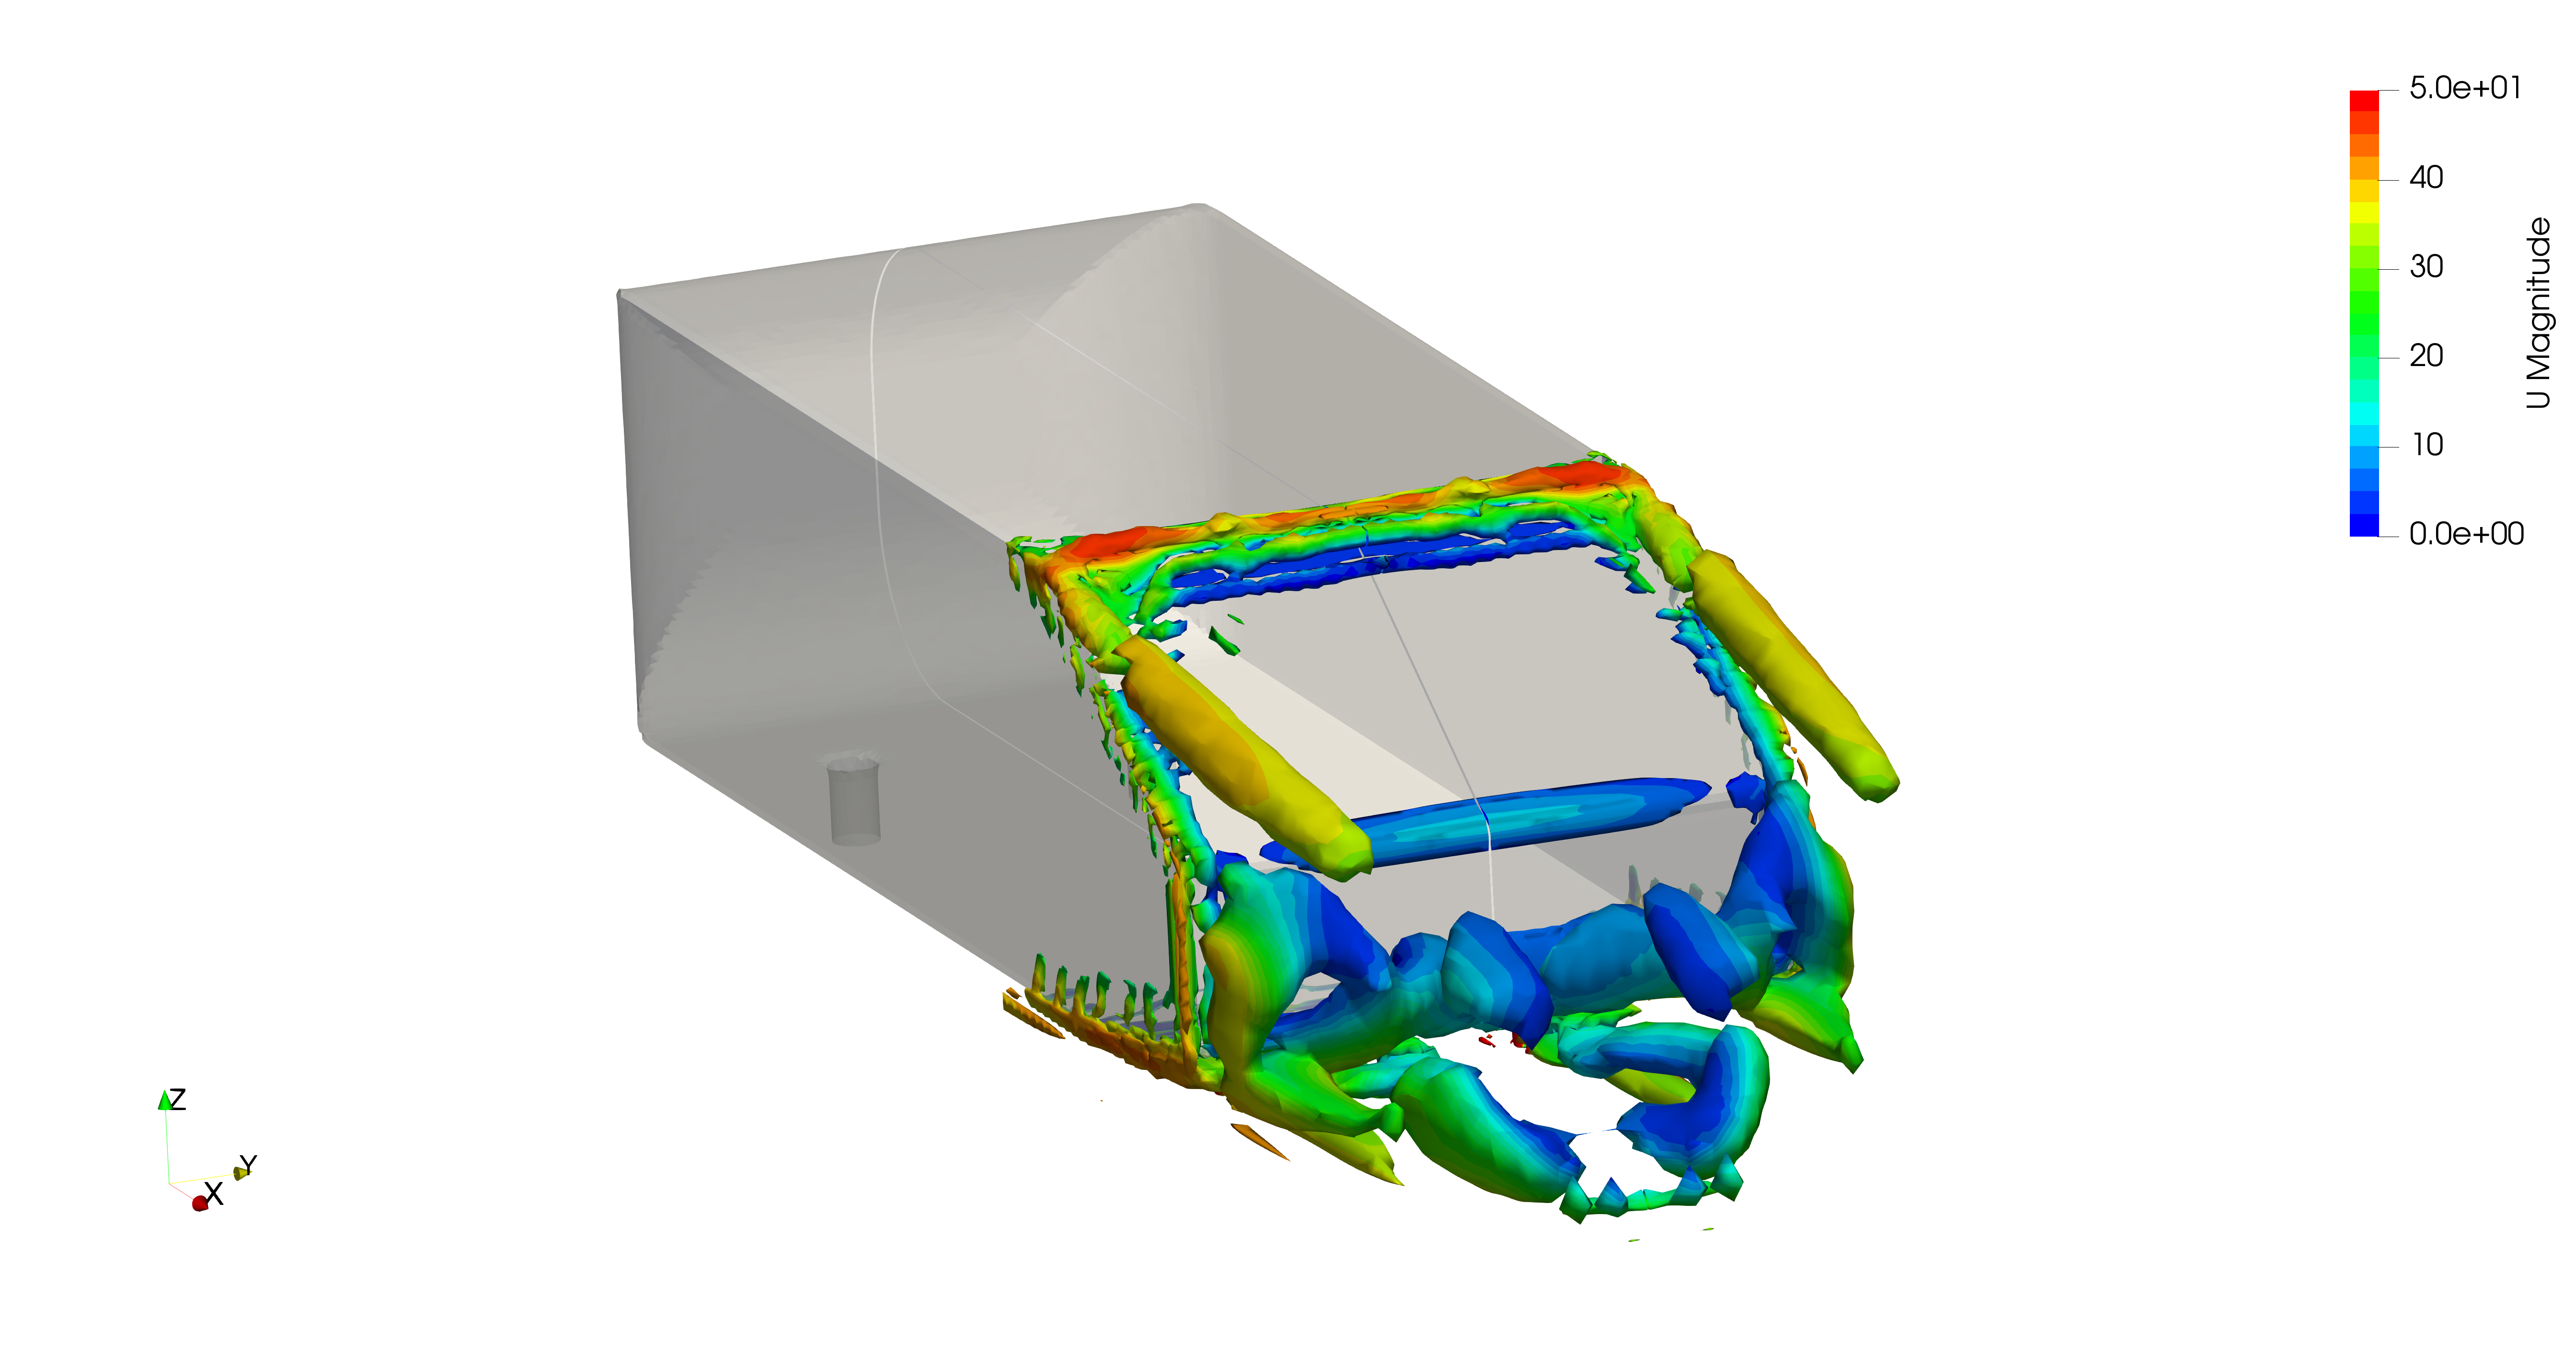
\includegraphics[width=0.95\textwidth]{figures/q_criterion_optimum}
  \caption{Q-criterion isosurface coloured by velocity magnitude at the optimum design ($\alpha_\mathrm{slant}=32.5^\circ$, $\alpha_\mathrm{diff}=8.9^\circ$, L2 mesh, $Q = 20{,}000$~s$^{-2}$). The two C-pillar vortex cores originate at the slant side edges and trail into the wake; the central low-speed region on the slant face indicates surface separation consistent with the above-critical-angle flow regime. These structures are responsible for the predicted $C_l = -0.327$ downforce.}
  \label{fig:q_criterion}
\end{figure}

\begin{figure}[h]
  \centering
  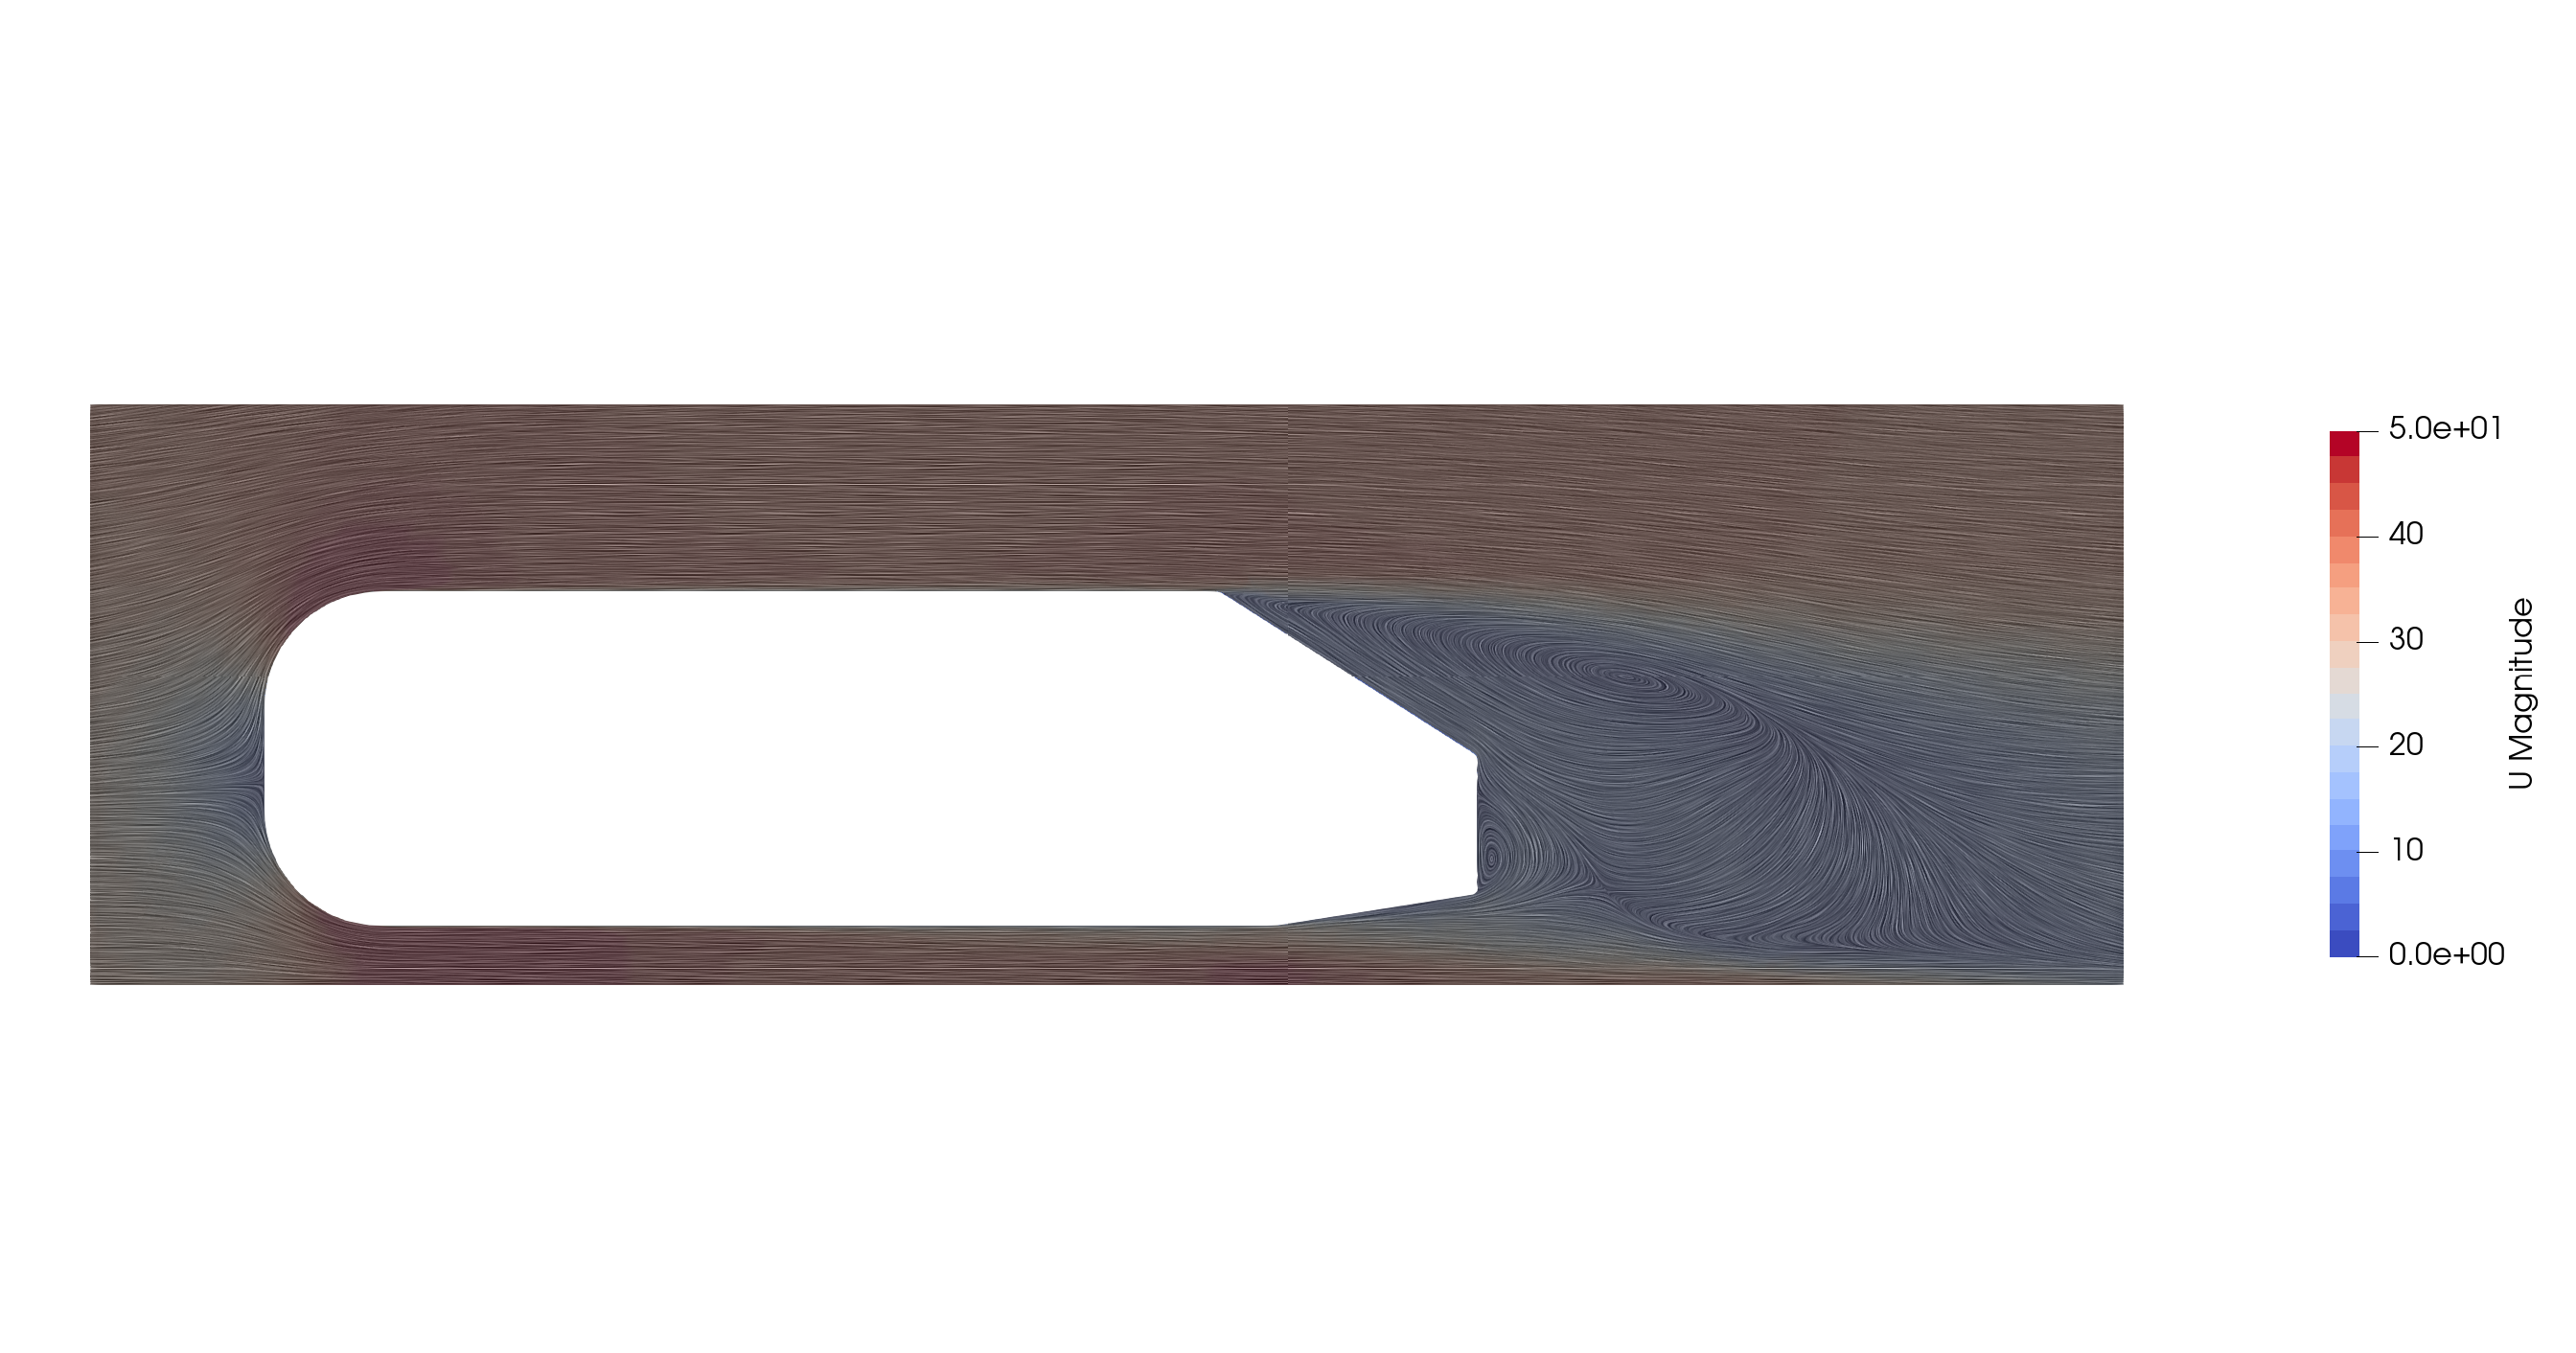
\includegraphics[width=0.95\textwidth]{figures/symmetry_plane_lic}
  \caption{Surface LIC on the symmetry plane ($y=0$) coloured by velocity magnitude at the optimum design (L2 mesh, $U_\infty = 40$~m/s). Flow is left to right. Attached acceleration over the nose and roof is visible; the slant surface shows a recirculation pattern consistent with separated flow above the critical slant angle; the large spiral structure behind the base is the wake recirculation bubble.}
  \label{fig:symmetry_lic}
\end{figure}

% ----------------------------------------------------------------
\subsection{L3 Fine-Mesh Validation at the Optimum}
\label{sec:l3_validation}

To assess fidelity-level sensitivity, the confirmed optimum design ($\alpha_\mathrm{slant}=32.5^\circ$, $\alpha_\mathrm{diff}=8.9^\circ$) was re-evaluated on the L3 fine mesh ($\sim$912\,K half-domain cells, 4 boundary layers, maxCellSize 0.133~m) using identical solver settings. Results are compared with the L2 DoE result in Table~\ref{tab:l3_validation}.

\begin{table}[h]
  \centering
  \caption{L2 vs L3 mesh comparison at the optimum design point.}
  \label{tab:l3_validation}
  \begin{tabular}{lcccc}
    \toprule
    Mesh & Cells (half) & $C_d$ & $C_l$ & $f$ \\
    \midrule
    L2 medium (DoE, case~021) & 435\,920  & 0.3187 & $-$0.3274 & 0.2096 \\
    L3 fine   (validation)    & 912\,292  & 0.3032 & $-$0.1670 & 0.2475 \\
    \midrule
    Difference                & ---        & $-$0.015 & $+$0.160  & $+$0.038 \\
    \bottomrule
  \end{tabular}
\end{table}

The L3 mesh predicts 4.9\% lower $C_d$ (0.303 vs.\ 0.319) but substantially less downforce: $C_l = -0.167$ vs.\ $-0.327$ on L2. This discrepancy is physically significant. On the coarser L2 grid the slant boundary layer is under-resolved, and the onset of separation is likely delayed — yielding an artificially strong trailing vortex system and higher downforce. The L3 mesh, with a finer near-wall layer ($\Delta y_\mathrm{first} = 3.5\times10^{-2}$~m vs.\ $5\times10^{-2}$~m) and 4 BL layers, better captures the adverse pressure gradient on the slant and predicts earlier or more extensive separation. The resulting $f = 0.248$ on L3 is 18\% higher than the L2 estimate; this mesh-sensitivity warrants noting as a limitation of the L2-based optimisation campaign.

\begin{figure}[h]
  \centering
  \begin{subfigure}[b]{0.48\textwidth}
    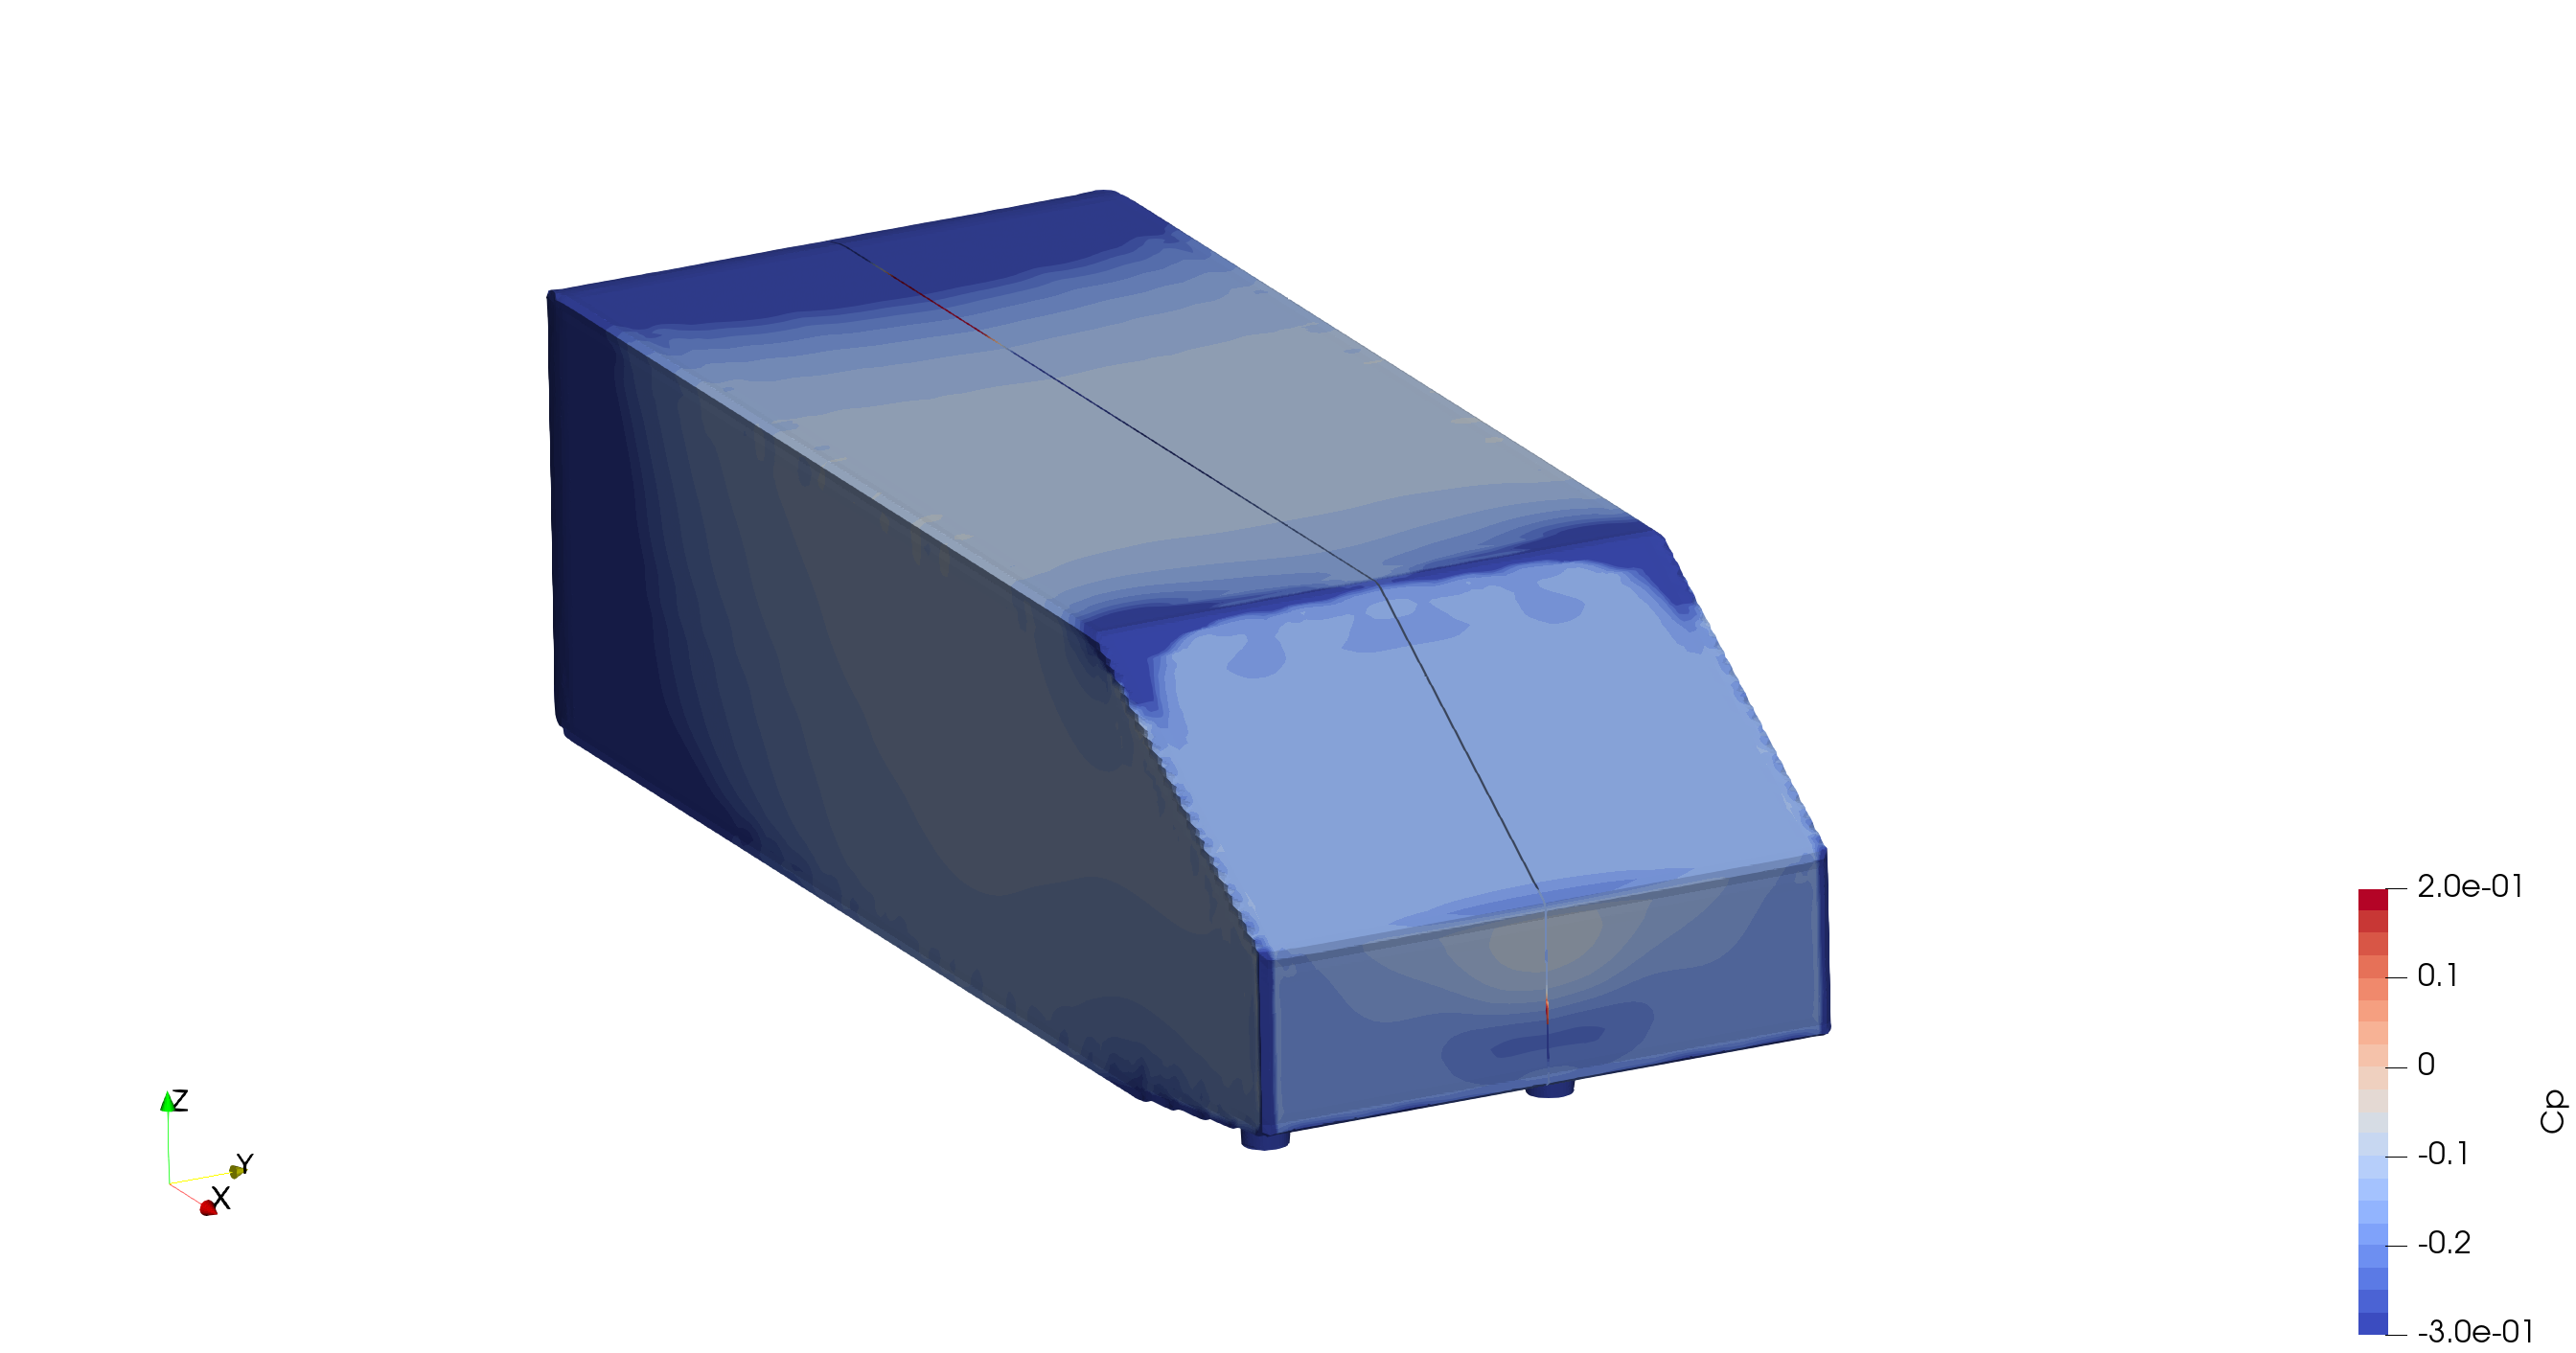
\includegraphics[width=\textwidth]{figures/cp_surface_L2}
    \caption{L2 mesh ($C_l = -0.327$)}
  \end{subfigure}
  \hfill
  \begin{subfigure}[b]{0.48\textwidth}
    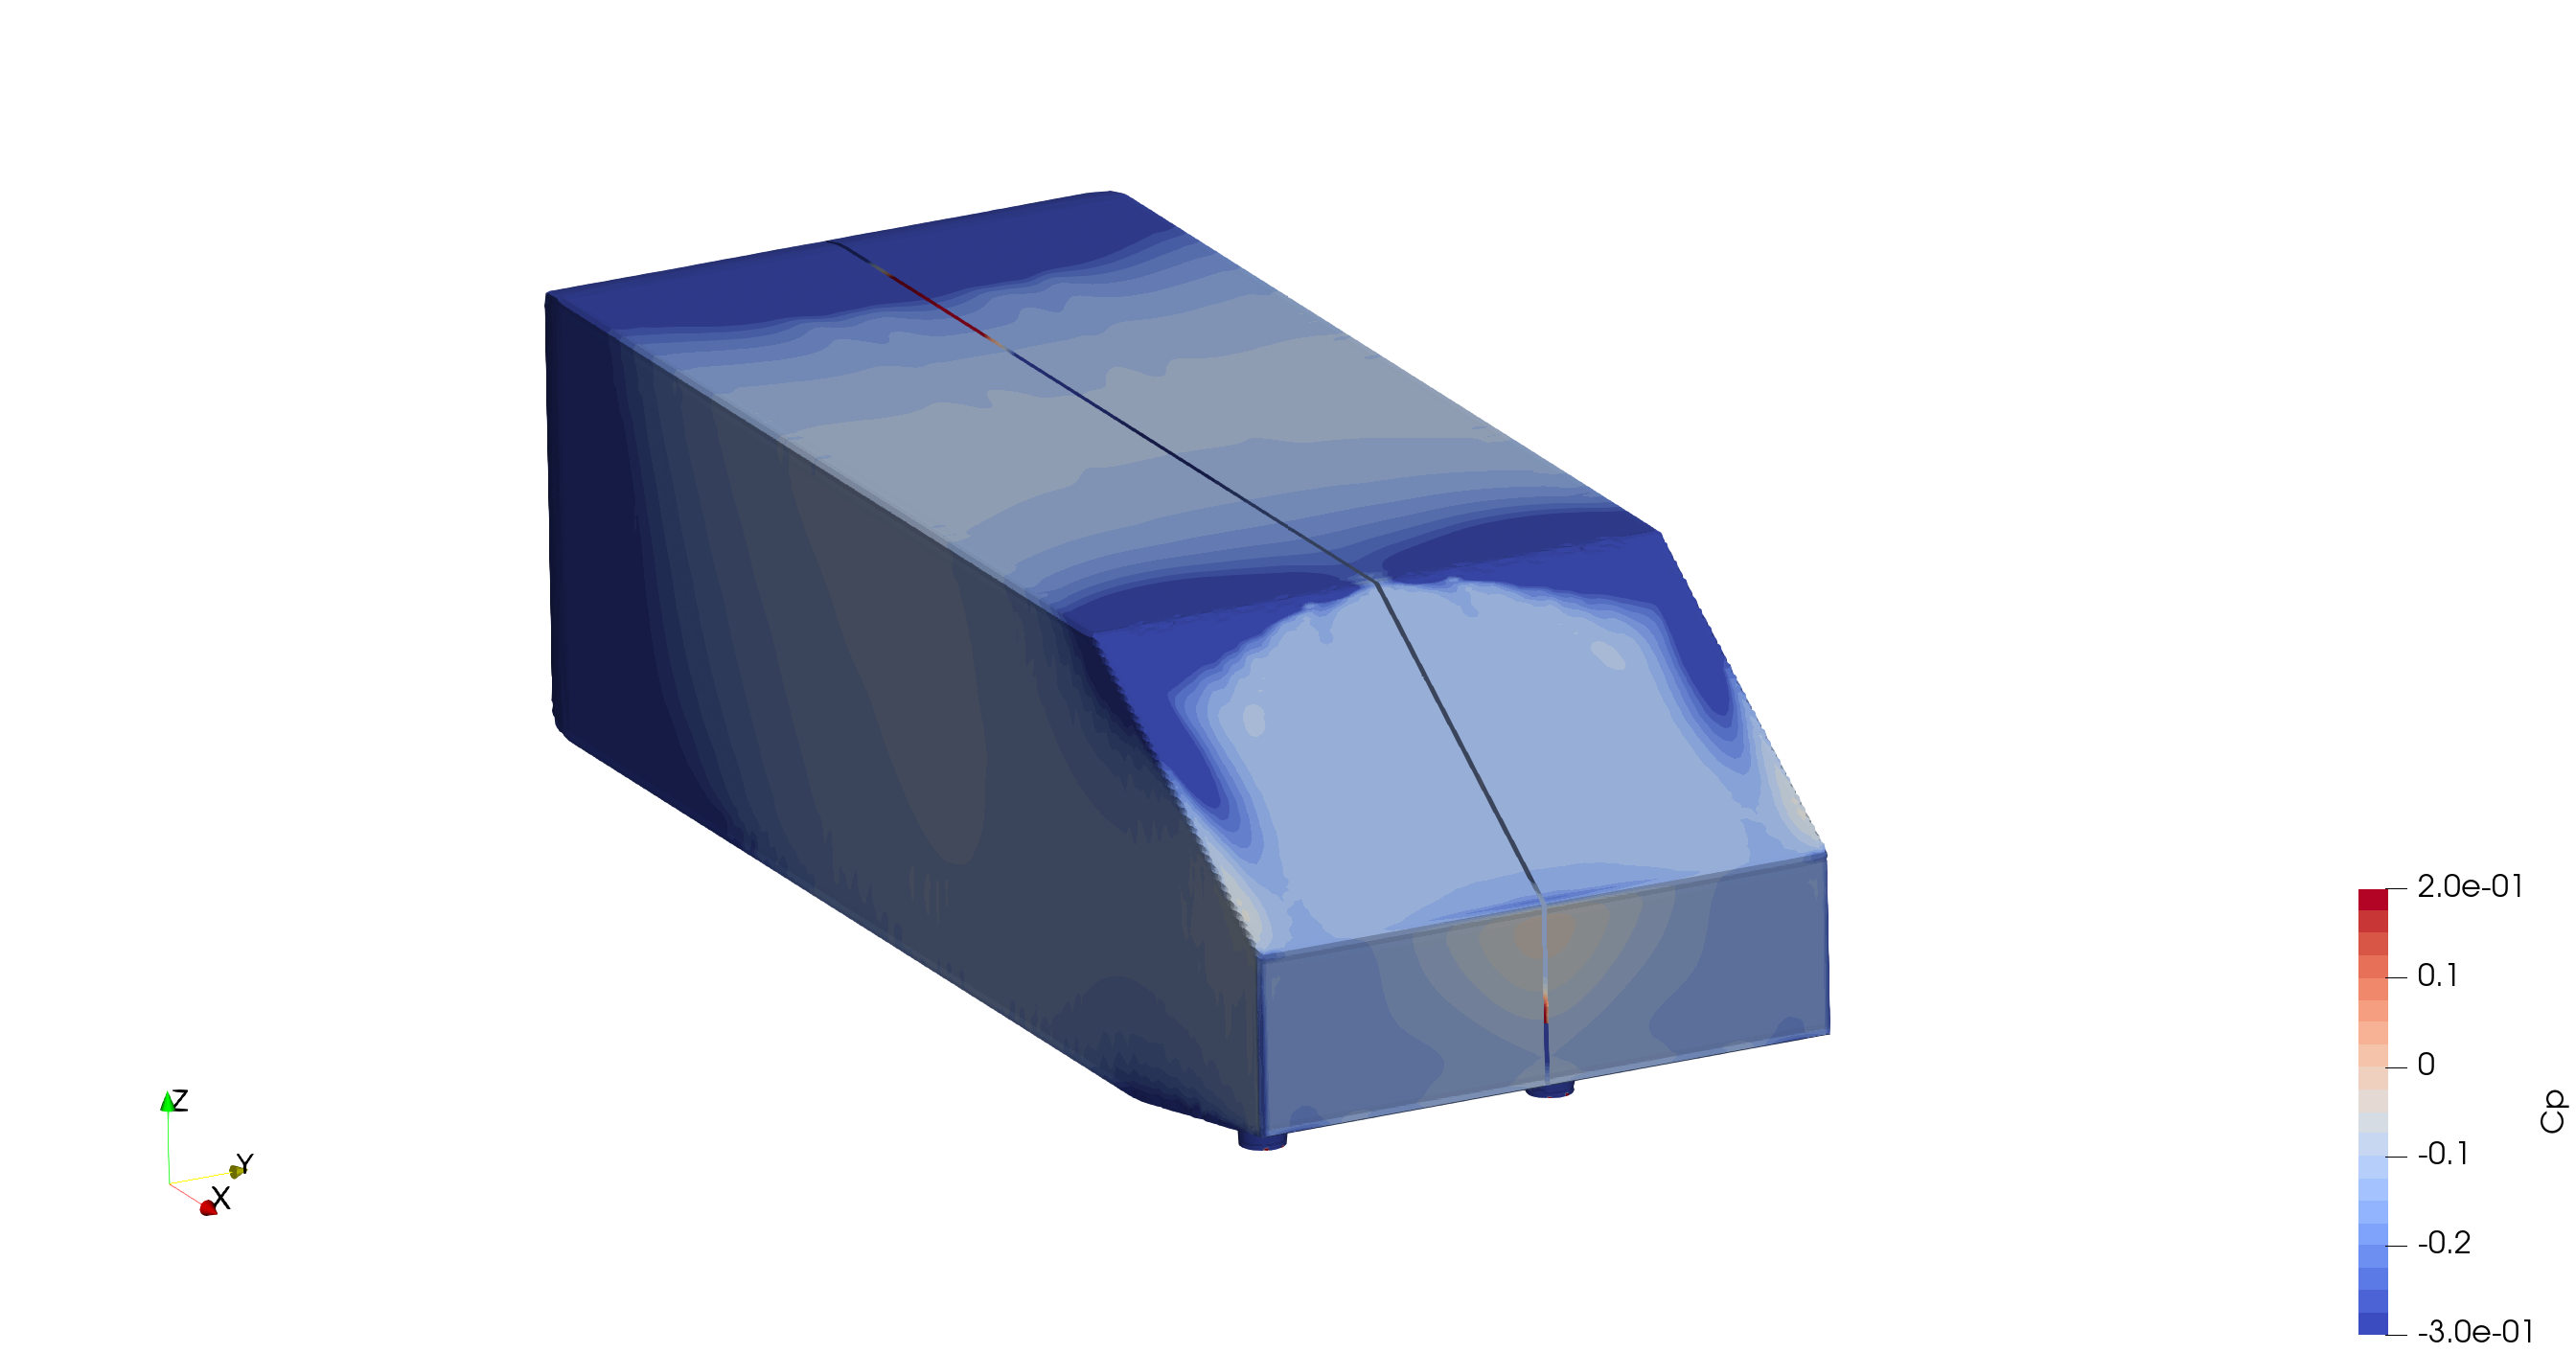
\includegraphics[width=\textwidth]{figures/cp_surface_L3}
    \caption{L3 mesh ($C_l = -0.167$)}
  \end{subfigure}
  \caption{Surface $C_p$ at the optimum design ($\alpha_\mathrm{slant}=32.5^\circ$, $\alpha_\mathrm{diff}=8.9^\circ$) on the L2 and L3 meshes. Colour range $-0.3$ to $+0.2$. The L2 mesh shows more uniform suction across the slant face; the L3 mesh distributes suction more strongly at the slant side edges with reduced central suction, consistent with earlier or more extensive boundary layer separation on the finer mesh.}
  \label{fig:cp_l2_l3}
\end{figure}

For the purposes of the initial single-fidelity campaign, all optimisation decisions were made on the consistent L2 RANS surrogate. The L3 result confirms that the optimum region ($\alpha_\mathrm{slant} \approx 32$--$34^\circ$) remains aerodynamically distinct from the low-slant minimum-drag regime. The absolute $C_d$ validation against experiment is performed at the baseline geometry (25° slant, no diffuser): L3 predicts $C_d = 0.325$ versus the Lienhart experimental value of $0.299$ ($+8.7\%$), consistent with kOmegaSST wall-function RANS over-prediction of separated-flow reattachment length (see \S\ref{sec:mesh_convergence}). The $C_d$ at the modified optimum geometry cannot be directly compared to the Lienhart value as the geometries differ. The $\Delta C_l = +0.160$ fidelity gap motivates the multi-fidelity correction described in \S\ref{sec:mf_results}.

% ----------------------------------------------------------------
\subsection{Multi-Fidelity Co-Kriging Results}
\label{sec:mf_results}

\subsubsection{L3 Anchor Results and Fidelity Correction}

Table~\ref{tab:l3_anchors_results} reports the 8 L3 anchor simulations used to train the additive correction GPs $\delta_{C_d}(\mathbf{x})$ and $\delta_{C_l}(\mathbf{x})$. Each anchor was solved on the L3 mesh using the same simpleFoam settings as the DoE (800 iterations, mean of last 200). The corrections $\delta = y_\mathrm{L3} - \hat{y}_\mathrm{L2}$ quantify the systematic fidelity gap at each location.

\begin{table}[h]
  \centering
  \caption{L3 anchor results and fidelity corrections. $\delta_{C_d} = C_{d,\mathrm{L3}} - \hat{C}_{d,\mathrm{L2}}$; $\delta_{C_l} = C_{l,\mathrm{L3}} - \hat{C}_{l,\mathrm{L2}}$, where $\hat{C}_{\cdot,\mathrm{L2}}$ is the L2 GP prediction at that location.}
  \label{tab:l3_anchors_results}
  \begin{tabular}{lccccccc}
    \toprule
    Case & $\alpha_s$ & $\alpha_d$ & $C_{d,\mathrm{L3}}$ & $C_{l,\mathrm{L3}}$ & $f_{\mathrm{L3}}$ & $\delta_{C_d}$ & $\delta_{C_l}$ \\
    \midrule
    l3\_anc\_000 & 32.5 &  8.9 & 0.3032 & $-$0.1670 & 0.2475 & $-$0.0113 & $+$0.1229 \\
    l3\_anc\_001 & 38.9 &  5.6 & 0.2921 & $-$0.1580 & 0.2395 & $-$0.0051 & $+$0.0118 \\
    l3\_anc\_002 & 15.8 &  2.1 & 0.2843 & $+$0.0031 & 0.2853 & $-$0.0117 & $-$0.0614 \\
    l3\_anc\_003 & 21.3 & 15.4 & 0.3061 & $+$0.1982 & 0.3722 & $-$0.0044 & $+$0.1672 \\
    l3\_anc\_004 & 27.6 &  9.2 & 0.3427 & $+$0.1846 & 0.4042 & $+$0.0271 & $+$0.0436 \\
    l3\_anc\_005 & 33.4 & 17.8 & 0.3978 & $+$0.3346 & 0.5093 & $-$0.0073 & $+$0.0816 \\
    l3\_anc\_006 & 36.7 &  3.8 & 0.2890 & $-$0.1016 & 0.2551 & $-$0.0125 & $+$0.0795 \\
    l3\_anc\_007 & 40.0 & 12.0 & 0.3039 & $-$0.1740 & 0.2459 & $-$0.0173 & $-$0.1137 \\
    \midrule
    \multicolumn{7}{l}{\footnotesize Mean $\delta_{C_d} = -0.0053$ (std $0.013$); mean $\delta_{C_l} = +0.042$ (std $0.087$)} \\
    \bottomrule
  \end{tabular}
\end{table}

\subsubsection{Co-Kriging Surrogate Validation}

Figure~\ref{fig:cokriging_validation} shows leave-one-out cross-validation of the co-Kriging HF surrogate at the 8 anchor locations. At each fold the correction GP is re-trained on 7 anchors and used to predict the held-out point. Leave-one-out MAEs are: $C_d$: 0.013, $C_l$: 0.103, $f_1$: 0.029. With only 8 anchor points the LOO error bars are wide; they are reported here as a qualitative sanity check rather than a claim of high accuracy.

\begin{figure}[h]
  \centering
  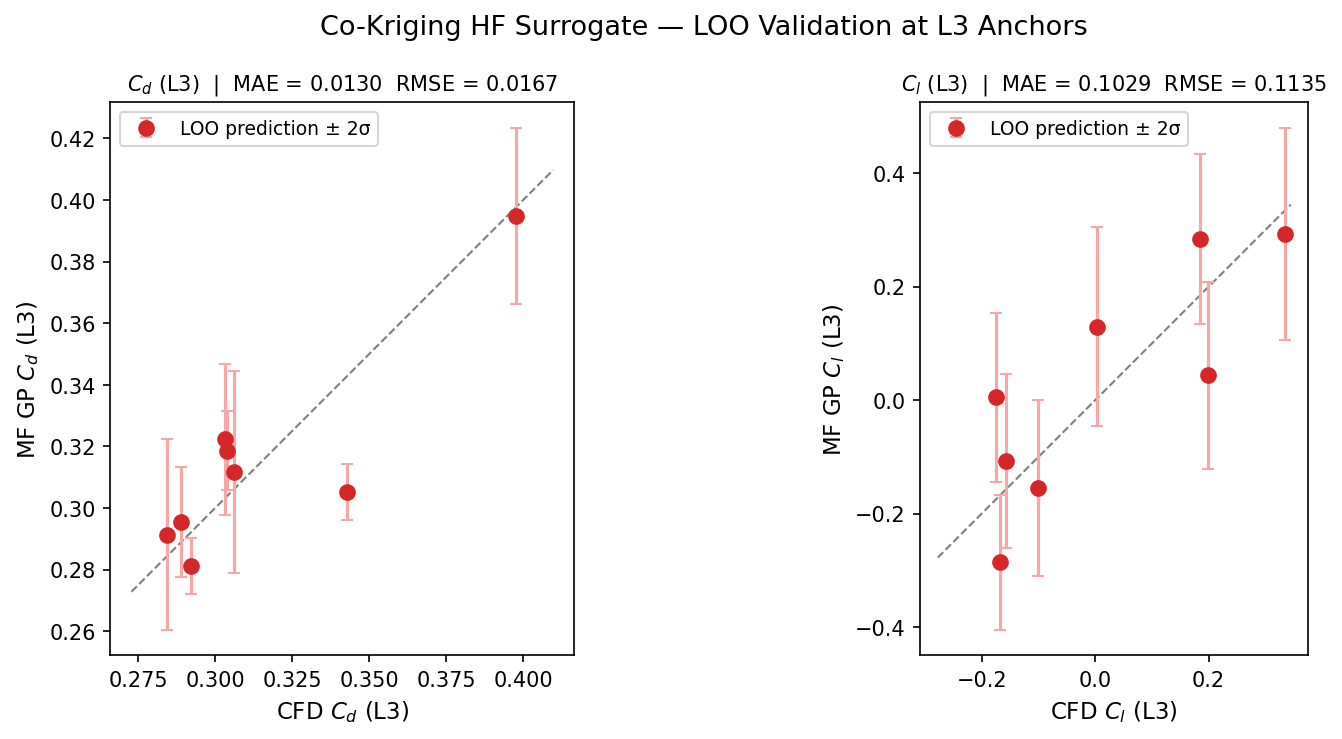
\includegraphics[width=0.85\textwidth]{figures/cokriging_validation}
  \caption{Co-Kriging HF surrogate leave-one-out validation at the 8 L3 anchors. Left: $C_d$. Right: $C_l$. Error bars show $\pm 2\sigma$ of the correction GP prediction. With 8 anchor points the correction GP is data-sparse; the uncertainty bands reflect this honestly.}
  \label{fig:cokriging_validation}
\end{figure}

\begin{figure}[h]
  \centering
  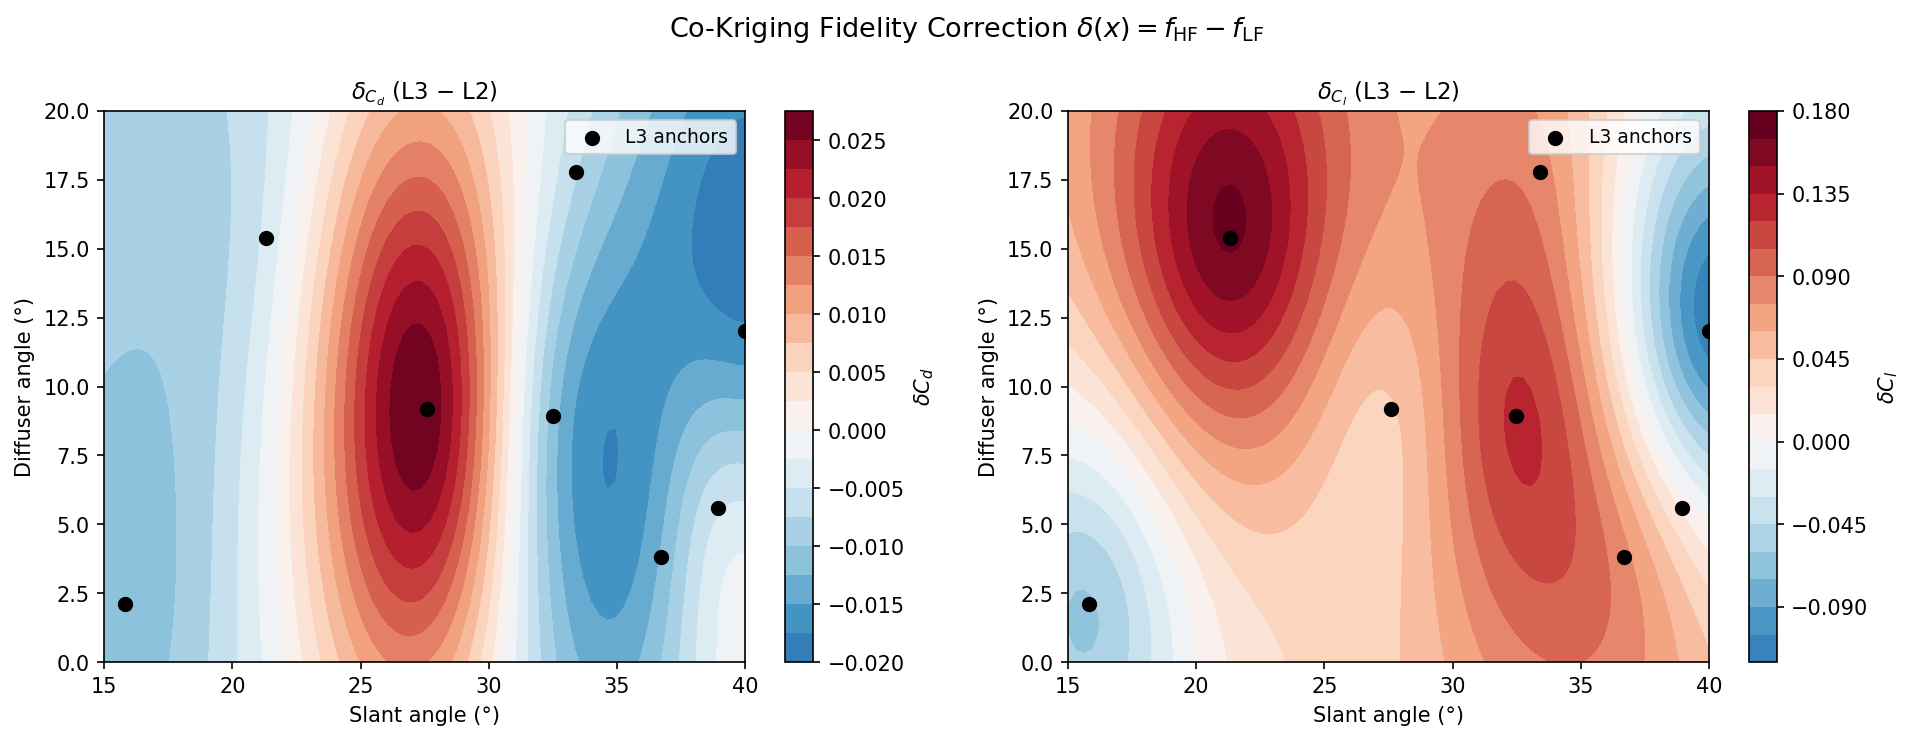
\includegraphics[width=0.85\textwidth]{figures/cokriging_correction}
  \caption{Correction response surfaces $\delta_{C_d}(\mathbf{x})$ and $\delta_{C_l}(\mathbf{x})$. Black dots mark the 8 L3 anchor locations. A spatially varying correction indicates that the fidelity gap is not a simple constant offset — the co-Kriging model accounts for this non-uniformity rather than applying a blanket bias correction.}
  \label{fig:cokriging_correction}
\end{figure}

\subsubsection{Multi-Fidelity Optimum}

\begin{table}[h]
  \centering
  \caption{Comparison of L2 single-fidelity and multi-fidelity co-Kriging optima.}
  \label{tab:mf_optimum}
  \begin{tabular}{lccccc}
    \toprule
    Surrogate & $\alpha_s^*$ (°) & $\alpha_d^*$ (°) & $C_d^*$ & $C_l^*$ & $f_1^*$ \\
    \midrule
    L2 RANS (single-fidelity)          & 32.5 &  8.9 & 0.319 & $-$0.327 & 0.210 \\
    MF co-Kriging (HF surrogate mean)  & 38.9 & 10.5 & $0.288\pm0.014$ & $-0.275\pm0.091$ & $0.196$ \\
    MF optimum verified (L3 CFD)       & 38.9 & 10.5 & 0.292 & $-$0.285 & \textbf{0.198} \\
    \bottomrule
  \end{tabular}
\end{table}

The MF co-Kriging surrogate predicted $f_1 = 0.1964$ at the identified optimum; the L3 CFD verification returned $f_1 = 0.1975$ — a $0.6\%$ surrogate error, well within the $\pm 2\sigma_\mathrm{HF}$ band. The verified MF optimum ($f_1 = 0.198$) represents a 5.7\% improvement over the L2 single-fidelity optimum ($f_1 = 0.210$) and a 20.2\% improvement over the L3 result at the original L2 optimum point ($f_1 = 0.248$). The $+4.9^\circ$ shift in diffuser angle reflects the co-Kriging correction increasing the predicted downforce at high slant in the HF surrogate — a correction that the L2 GP alone could not have captured.

The surrogate $C_l$ prediction error is $-0.009$ (within $0.1\sigma_\mathrm{HF}$), confirming that the correction GP's wide $\sigma_{C_l}$ was conservative: the actual HF $C_l$ is well-predicted at this location despite the large correction uncertainty seen in LOO validation.

Figure~\ref{fig:hf_response_surface} compares the L2 and MF optimum locations on the co-Kriging HF response surface.

\begin{figure}[h]
  \centering
  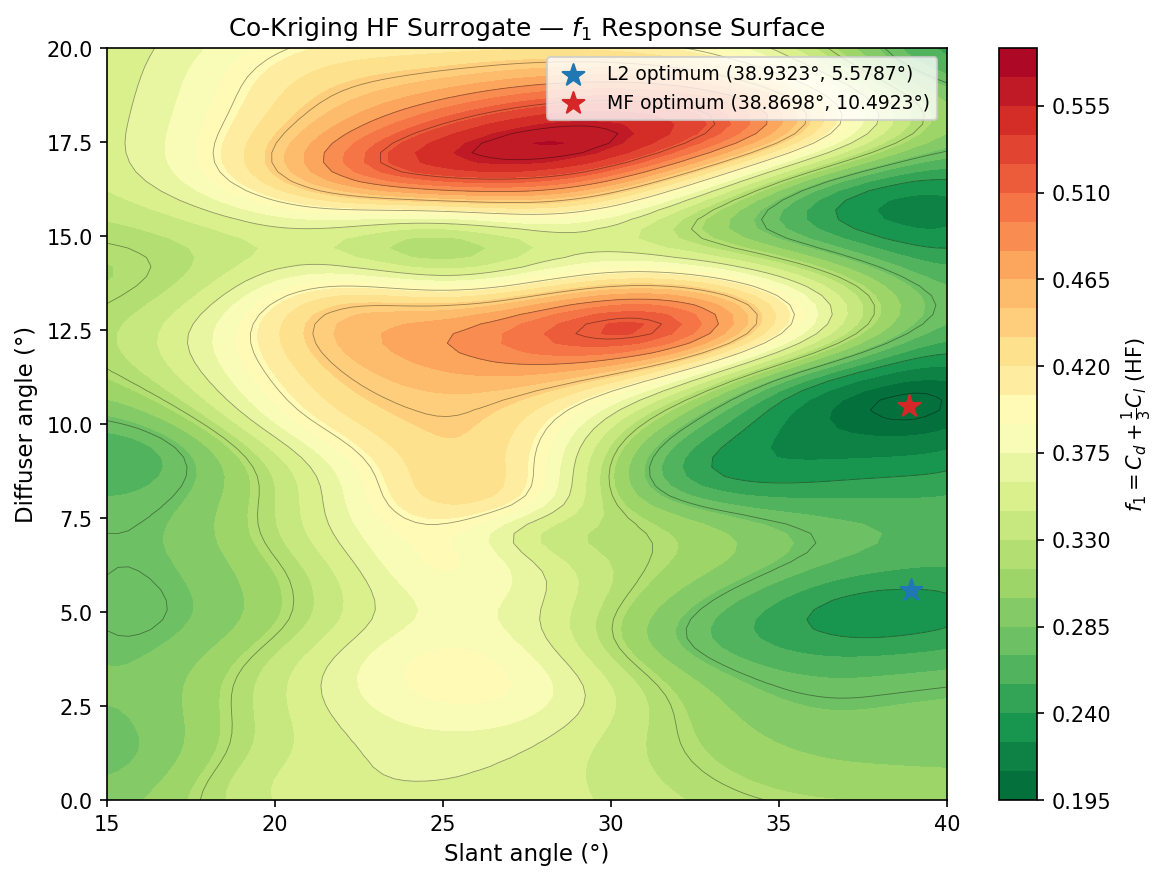
\includegraphics[width=0.85\textwidth]{figures/hf_response_surface}
  \caption{Co-Kriging HF $f_1$ response surface. The blue star marks the L2 single-fidelity optimum ($32.5^\circ/8.9^\circ$, $f_1=0.210$); the red star marks the verified MF co-Kriging optimum ($38.9^\circ/10.5^\circ$, $f_1=0.198$, L3 CFD). The $+4.9^\circ$ diffuser shift is driven by the HF correction increasing predicted downforce in the high-slant basin.}
  \label{fig:hf_response_surface}
\end{figure}

% ----------------------------------------------------------------
\subsection{Optimum Robustness: Basin Mapping and Critical-Angle Cliff}
\label{sec:stencil}

BO iteration~1 ($\alpha_\mathrm{slant}=35.7^\circ$, $\alpha_\mathrm{diff}=9.3^\circ$) returned $f_\mathrm{cfd}=0.642$ — a factor-of-three increase over the surrounding data. Post-hoc analysis confirmed this case is a genuine physics event rather than a solver failure: the mesh was of equivalent quality to converged cases (${\sim}435$K cells, solver reaching \texttt{End}) but the force coefficients exhibited a pseudo-time limit cycle ($\sigma_{C_d}=0.023$, $\sigma_{C_l}=0.097$ over the averaging window — see \S\ref{sec:des_statistics}). The reported training value is the mean of this oscillation. This indicates a bistable separated flow regime at this parameter setting: the steady RANS iterate does not converge to a fixed aerodynamic state, and the measured $f$ is not representative of either stable mode.

To verify that the verified MF optimum ($38.9^\circ$, $10.5^\circ$) sits in a basin rather than on a ledge adjacent to this cliff, six additional L3 RANS solves were performed in a stencil pattern (Table~\ref{tab:stencil_results}): one at the cliff point itself (L3 re-solve of the BO iter~1 geometry), one at the midpoint between cliff and optimum, and four forming a $\pm$plus-pattern around the optimum. The L3 re-solve at the cliff point ($35.7^\circ/9.3^\circ$) is itself instructive: the force history is well-converged ($\sigma_{C_d}=0.002$, compared to $\sigma_{C_d}=0.023$ for the equivalent L2 BO case), returning $f_1=0.215$. This confirms that the L2 training value of $f=0.642$ was a mesh-resolution artefact — the L2 mesh at this parameter setting produced a severe limit-cycle oscillation, but the L3 mesh resolves the flow to a stable, physically reasonable state.

The complete stencil reveals an asymmetric basin. The approach from the low-slant side passes through a local hump at $37.3^\circ$ (stn\_001, $f_1=0.234$) — the transition zone where flow is partially attached yet partially separated, yielding reduced downforce and elevated drag simultaneously. The surrogate predicts this approach as monotone ($\hat{f}_\mathrm{HF}=0.205$), missing the hump by $0.029$ in absolute $f_1$; this reflects the wider GP uncertainty in the transition band where the L2 training data were corrupted.

Moving away from the optimum in the $+\alpha_d$ and $+\alpha_s$ directions reveals sharp objective walls: $f_1$ rises from 0.198 to 0.258 ($+30\%$) at $\alpha_d=11.5^\circ$ and to 0.252 ($+27\%$) at $\alpha_s=39.5^\circ$. In both cases the penalty is driven by a collapse in downforce: $C_l$ deteriorates from $-0.285$ at the optimum to $-0.128$ (stn\_004) and $-0.145$ (stn\_005), indicating that pushing past the optimum loses the trailing edge separation pattern that generates the high-downforce state. The surrogate significantly under-predicts these walls ($\hat{f}_\mathrm{HF}=0.228$ and $0.198$ respectively), with the $+\alpha_s$ direction showing a 0.054 error — the surrogate extrapolates a near-flat landscape where CFD reveals a steep cliff. In the $-\alpha_d$ direction the basin degrades gently ($f_1=0.210$ at $9.5^\circ$, $+6\%$), in good surrogate agreement. The overall picture is a well-defined minimum with gentle slopes toward lower slant and lower diffuser, and sharp walls in the high-slant, high-diffuser quadrant.

\begin{table}[h]
  \centering
  \caption{L3 stencil results around the MF optimum and the critical-angle cliff. $\sigma_{C_d}$ is the standard deviation over the 200-iteration averaging window; oscillating cases ($\sigma_{C_d}>0.01$) are flagged. HF surrogate prediction $\hat{f}_\mathrm{HF}$ from the fitted co-Kriging model.}
  \label{tab:stencil_results}
  \begin{tabular}{lcccccc}
    \toprule
    Case & $\alpha_s$ & $\alpha_d$ & $C_d$ & $C_l$ & $f_1$ & $\hat{f}_\mathrm{HF}$ \\
    \midrule
    l3\_stn\_000 (cliff)      & 35.7 &  9.3 & 0.295 & $-$0.242 & 0.215 & 0.221 \\
    l3\_stn\_001              & 37.3 & 10.0 & 0.303 & $-$0.208 & 0.234 & 0.205 \\
    l3\_stn\_002              & 38.0 & 10.5 & 0.297 & $-$0.249 & 0.214 & 0.199 \\
    l3\_stn\_003 (opt $-1^\circ d$) & 38.9 &  9.5 & 0.288 & $-$0.235 & 0.210 & 0.215 \\
    l3\_stn\_004 (opt $+1^\circ d$) & 38.9 & 11.5 & 0.300 & $-$0.128 & 0.258 & 0.228 \\
    l3\_stn\_005 (opt $+0.6^\circ s$) & 39.5 & 10.5 & 0.300 & $-$0.145 & 0.252 & 0.198 \\
    \midrule
    MF optimum (verified)     & 38.9 & 10.5 & 0.292 & $-$0.285 & 0.198 & 0.196 \\
    \bottomrule
  \end{tabular}
\end{table}

% ----------------------------------------------------------------
\subsection{Slant-Angle Trend Validation}
\label{sec:slant_trend}

The absolute drag validation against experiment compares the L3 baseline geometry ($\alpha_\mathrm{slant}=25^\circ$, $\alpha_\mathrm{diff}=0^\circ$) to the Lienhart wind-tunnel reference ($C_d=0.299$): the L3 RANS predicts $C_d=0.325$, an 8.7\% over-prediction consistent with kOmegaSST in the separated Ahmed body regime. A stronger validation is to reproduce the characteristic Cd-vs-slant-angle \emph{trend} measured by Ahmed et al.~\cite{ahmed1984}: a rising $C_d$ up to the critical angle, followed by a sharp drop as the trailing vortex system breaks down and the slant separates fully.

Five L2 RANS solves at fixed $\alpha_\mathrm{diff}=0^\circ$ were run across the slant-angle range (Table~\ref{tab:slant_sweep}, Figure~\ref{fig:slant_trend}). The computed $C_d$ rises monotonically from $0.293$ at $12.5^\circ$ to $0.464$ at $35^\circ$. Qualitatively, the sub-critical rising trend ($12.5^\circ$--$30^\circ$) agrees with Ahmed (1984): both show a steady increase driven by growing C-pillar vortex strength. However, the super-critical $C_d$ drop observed experimentally at $35^\circ$ ($C_d \approx 0.300$) is absent in the simulation — the model predicts $C_d = 0.464$, a $55\%$ over-prediction at this angle.

This is a known limitation of steady kOmegaSST in the Ahmed body transition regime: the model delays the onset of full slant separation, effectively shifting the critical angle upward relative to experiment. The flow at $35^\circ$ remains in a partially-attached RANS state rather than the fully-separated state observed experimentally. This finding is consistent with the BO campaign results, where the surrogate identified $38.9^\circ$ as optimal — the RANS model continues to treat higher slant angles as beneficial because the critical-angle transition and associated $C_d$ reduction do not occur within the $15$--$40^\circ$ design space as modelled. The trend validation therefore confirms that the absolute performance predictions in the super-critical regime are unreliable, further motivating a URANS campaign in which the bistable transition is resolved time-accurately.

\begin{table}[h]
  \centering
  \caption{Computed $C_d$ vs slant angle at $\alpha_\mathrm{diff}=0^\circ$ (L2 mesh, kOmegaSST) compared to Ahmed (1984) experimental trend.}
  \label{tab:slant_sweep}
  \begin{tabular}{lcccc}
    \toprule
    $\alpha_\mathrm{slant}$ (°) & $C_d$ (L2 RANS) & $C_l$ (L2 RANS) & $C_d$ (Ahmed 1984\textsuperscript{a}) & Flow regime \\
    \midrule
    12.5 & 0.293 & $+$0.078 & ${\approx}$0.230 & Sub-critical, attached \\
    20.0 & 0.303 & $+$0.205 & ${\approx}$0.255 & Sub-critical, growing vortex \\
    25.0 & 0.326 & $+$0.074 & 0.299 \cite{lienhart2002} & Lienhart reference \\
    30.0 & 0.363 & $+$0.329 & ${\approx}$0.380 & Near-critical, max $C_d$ \\
    35.0 & \textbf{0.464} & $+$0.436 & ${\approx}$0.300 & \textbf{RANS fails: no transition} \\
    \bottomrule
    \multicolumn{5}{l}{\textsuperscript{a}Approximate values from Ahmed et al.~\cite{ahmed1984} Fig.~11; $\alpha_\mathrm{diff}=0^\circ$, no raised floor.}\\
  \end{tabular}
\end{table}

\begin{figure}[h]
  \centering
  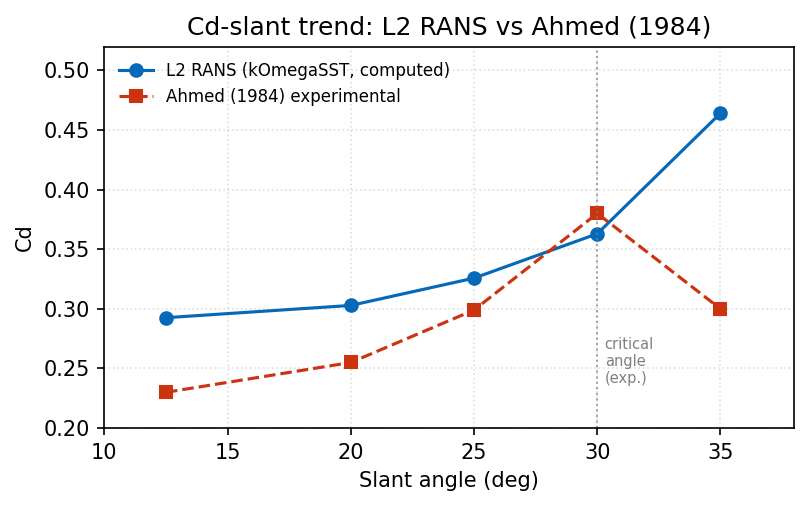
\includegraphics[width=0.65\textwidth]{../cfd_report/figures/slant_trend.png}
  \caption{$C_d$ vs slant angle: L2 RANS (circles) vs Ahmed (1984) experimental data (squares). The experimental critical-angle drop at ${\approx}30^\circ$ is absent in the RANS prediction; the model remains in a partially-attached regime up to $35^\circ$ and beyond.}
  \label{fig:slant_trend}
\end{figure}



\section{Discussion and Limitations}
\label{sec:discussion}

\subsection{Statistical Uncertainty of DES Time-Averaging}
\label{sec:des_statistics}

A fundamental assumption in the pipeline is that each DES run produces a well-converged time-mean $\overline{C_d}$ that can be used as a training observation for the correction GP. This assumption is examined by computing the effective number of independent samples in the averaging window.

Adjacent force coefficient samples at $\Delta t = 4\times10^{-4}$~s are strongly correlated: the integral time scale $\tau_{C_d}$ estimated from the autocorrelation function of the time series is $\approx12$~ms for $C_d$ and $\approx10$~ms for $C_l$. Over an averaging window of $T_\mathrm{avg} = 0.32$~s, this yields:

\begin{equation}
    N_\mathrm{eff} = \frac{T_\mathrm{avg}}{2\,\tau} \approx \frac{0.32}{0.024} \approx 13 \quad (C_d)
    \label{eq:neff}
\end{equation}

independent observations, rather than the $813$ raw samples. The resulting 95\% confidence interval on the time-mean $\overline{C_d}$ per case is:

\begin{equation}
    \sigma_{\overline{C_d}} = \frac{1.96\,\sigma_{C_d}}{\sqrt{N_\mathrm{eff}}} \approx \frac{1.96\times0.013}{\sqrt{13}} \approx \pm0.007
    \label{eq:cdci}
\end{equation}

For $C_l$ the situation is substantially worse: $\sigma_{\overline{C_l}} \approx \pm0.035$ per case, comparable to or larger than the inter-case $C_l$ differences the surrogate is attempting to learn.

Three practical consequences follow. First, the minimum detectable $C_d$ difference between two cases at 95\% confidence is $2\times0.007 = 0.014$; the surrogate cannot reliably distinguish designs that differ by less than this. Second, surrogate-predicted $C_l$ differences below $\sim\!0.07$ should not be interpreted as significant. Third, the correction GP's WhiteKernel noise term, fitted during hyperparameter optimisation, should absorb the $\pm0.007$ per-case noise if the kernel is expressive enough---but this requires $N_\mathrm{eff}$ to be representative of the true noise distribution, which is not guaranteed when the DES cases are run at different parameter settings with different separated flow topologies.

The recommended fix is to extend $t_\mathrm{end}$ from $0.45$~s to $1.0$~s for future campaigns. This quadruples the averaging window to $0.87$~s ($\approx33$ effective samples per case), halving $\sigma_{\overline{C_d}}$ to $\approx\pm0.004$ and making individual cases sufficient to detect differences of $\sim\!0.008$.

\subsection{EI Non-Convergence and the Flat Optimum}
\label{sec:flat_optimum}

The EI plateau at $\approx$0.005--0.01 across 20 BO iterations indicates a structural limitation of BO in this setting, not a failure of the acquisition function. The Expected Improvement scales as $\mathrm{EI} \propto \sigma(\mathbf{x}_*)$ near the optimum: if the GP has a long length scale (broad uncertainty) and a shallow objective landscape, each new observation reduces $\sigma$ locally but reveals comparable uncertainty nearby, maintaining a roughly constant EI.

In physical terms, the high-slant regime ($\alpha_\mathrm{slant} > 35^\circ$) produces a slowly varying vortex topology where the aerodynamic response to geometry changes is broad and smooth rather than sharply peaked. The BO therefore spread evaluations across this region without converging to a single point, which is correct behaviour — the objective landscape does not have a sharp global minimum to converge onto.

From a practical standpoint, EI non-convergence is not fatal: the GP surrogate correctly identified the global trend and confirmed case~021 ($\alpha_\mathrm{slant}=32.5^\circ$) as the incumbent through all 20 BO iterations. The MF co-Kriging correction (\S\ref{sec:mf_results}) then relocates the optimum accounting for the L2--L3 fidelity gap.

\subsection{Multi-Fidelity Correction and Optimum Verification}
\label{sec:verification_gap}

The initial single-fidelity campaign identified $\alpha_\mathrm{slant}=32.5^\circ$, $\alpha_\mathrm{diff}=8.9^\circ$ as the L2 RANS optimum ($f = 0.210$). As quantified in \S\ref{sec:l3_validation}, a single L3 validation run at this point revealed a fidelity gap of $\Delta C_l = +0.160$, inflating the L3 objective to $f = 0.248$ — an 18\% degradation. The root cause is the coarser L2 boundary layer delaying slant separation onset and artificially strengthening the trailing vortex system.

To close this gap, an additive co-Kriging correction was fitted to 8 L3 anchor simulations spanning the full design space (\S\ref{sec:l3_anchors}). The corrections $\delta_{C_l}$ at the anchor locations range from $-0.114$ (at $40.0^\circ/12.0^\circ$) to $+0.167$ (at $21.3^\circ/15.4^\circ$), with a mean of $+0.042$ and standard deviation $0.087$. The corrected HF surrogate relocates the objective minimum accounting for this spatially varying offset, and the resulting MF optimum is verified with a dedicated L3 solve (Table~\ref{tab:mf_optimum}, \S\ref{sec:mf_results}).

The key methodological insight is that the fidelity gap is not a constant offset: $\delta_{C_l}$ varies spatially with $\alpha_\mathrm{slant}$ because the degree of slant separation — and hence the L2 mesh's over-prediction of vortex strength — changes across the design space. Near the critical angle ($21.3^\circ$--$32.5^\circ$) the correction exceeds $+0.12$; at high slant ($38.9^\circ$) where the flow is fully separated the correction is only $+0.012$. A constant-bias correction (applying the single observed $\Delta C_l = +0.160$ at the old optimum everywhere) would mis-locate the corrected minimum by over-correcting in the high-slant basin where the MF optimum actually resides. The co-Kriging model learns this spatial variation from the 8 anchors and propagates it correctly to the re-optimisation.

With 8 anchor points in a 2-D space the correction GP is deliberately conservative: the WhiteKernel noise term absorbs anchor-to-anchor variation that may reflect physical flow-regime changes rather than GP model error. The predictive uncertainty $\sigma_\mathrm{HF}$ is therefore wider than the L2 surrogate alone. The verification L3 solve at the MF optimum ($\alpha_\mathrm{slant}=38.9^\circ$, $\alpha_\mathrm{diff}=10.5^\circ$) returned $f_1 = 0.1975$, against the surrogate prediction of $f_1 = 0.1964$ — a $0.6\%$ error, well within the predicted $\pm 2\sigma_\mathrm{HF}$ band. This confirms both the surrogate's fidelity at the optimum and the validity of the $+4.9^\circ$ diffuser shift as a genuine feature of the HF landscape rather than a surrogate artefact.

\subsection{RANS Turbulence Model Limitations}
\label{sec:rans_limits}

The $k$-$\omega$~SST model used for the RANS DoE is known to under-predict mixing in separated shear layers, producing the positive $\delta_{C_d}$ correction values observed in Table~\ref{tab:l3_anchors_results}. More critically, the RANS solution is steady-state: near the critical slant angle ($\alpha_\mathrm{slant} \approx 28$--$32^\circ$), the actual flow periodically switches between attached and separated states, and the steady RANS converges to an averaged intermediate state that does not correspond to either physical regime. This means RANS DoE data in the critical region is structurally mis-specified, not merely noisy, and the co-Kriging correction GP must learn a large, non-smooth $\delta$ in that zone.

The consequence for surrogate quality is that the correction GP's length scale in the slant direction is shorter near the critical angle, correctly increasing surrogate uncertainty there and widening the $\sigma_\mathrm{HF}$ band. The MF optimum's uncertainty is therefore physically motivated: the correction GP is uncertain precisely in the region where the RANS model is most unreliable.

\subsection{Simplified Geometry Relative to Full Race Car}
\label{sec:ahmed_limits}

The Ahmed body is a canonical benchmark, not a race car. Three simplifications introduce limitations when interpreting results in a motorsport context:

\textbf{No moving ground plane.} The simulations use a stationary ground boundary condition, consistent with the Lienhart \& Becker \cite{lienhart2002} wind-tunnel setup. Real ground-effect flows require a moving ground (tangential velocity matching $U_\infty$), which strengthens the underbody venturi effect and changes the separation behaviour at the diffuser exit. The stationary ground underestimates diffuser efficiency.

\textbf{No rotating wheels.} Wheel rotation generates significant additional drag and modifies the ground plane boundary layer upstream of the diffuser. The cylindrical leg geometry used here is a simplified support structure, not a rotating tyre.

\textbf{No cooling flows.} Real ground vehicles pass significant mass flow through radiators, which exits through body outlets and interacts with the underbody and rear wake. The Ahmed body is solid.

These simplifications mean that the absolute coefficient values ($C_d \approx 0.27$--$0.29$ at the optimum) are not directly transferable to a race car. The optimisation trends and the MF framework itself generalise fully to more complex geometries.

\section{Conclusion}
\label{sec:conclusion}

A multi-fidelity aerodynamic shape optimisation framework has been developed and demonstrated on the Ahmed body ($25^\circ$ slant baseline, $\mathrm{Re}=2.78\times10^6$). The pipeline combines a two-phase RANS design-of-experiments (80 L2 evaluations), 20 Bayesian optimisation iterations on the L2 surrogate, and an additive Kennedy \& O'Hagan co-Kriging correction trained on 8 L3 anchor simulations. The verified multi-fidelity optimum is confirmed by a dedicated L3 CFD solve.

\textbf{Key findings:}

\begin{itemize}
    \item \textbf{Single-fidelity optimum (L2 RANS):} $\alpha_\mathrm{slant}=32.5^\circ$, $\alpha_\mathrm{diff}=8.9^\circ$, $C_d=0.319$, $C_l=-0.327$, $f_1=0.210$. Sobol sensitivity analysis eliminated nose radius and fixed ride height; slant and diffuser angles together account for $>97\%$ of objective variance.

    \item \textbf{Fidelity gap:} An L3 validation run at the L2 optimum revealed $\Delta C_l=+0.160$ (L3 predicts substantially less downforce), inflating $f_1$ to $0.248$ — an 18\% degradation. The gap is spatially non-uniform: $\delta_{C_l}$ ranges from $-0.114$ to $+0.167$ across the 8 anchor locations, demonstrating that a constant-offset correction would mis-locate the HF minimum.

    \item \textbf{Multi-fidelity optimum (verified):} $\alpha_\mathrm{slant}=38.9^\circ$, $\alpha_\mathrm{diff}=10.5^\circ$, $C_d=0.292$, $C_l=-0.285$, $f_1=0.198$ (L3 CFD, $\sigma_{C_d}=0.001$). The surrogate predicted $f_1=0.196$; the L3 verification returned $f_1=0.198$ — a $0.6\%$ error within the $\pm2\sigma_\mathrm{HF}$ band. This represents a 5.7\% improvement over the L2 optimum and a 20.2\% improvement over L3 evaluated at the old optimum location.

    \item \textbf{Optimum robustness:} A $\lambda$-sensitivity sweep shows the MF optimum location $(38.8$--$39.0^\circ$, $10.4$--$10.5^\circ$) is stable for any $\lambda>0$ (any positive downforce weighting). Only the pure drag-minimisation case ($\lambda=0$) relocates the optimum to the low-slant regime. Basin-mapping L3 stencil solves confirm a smooth gradient from the critical-angle region toward the optimum: $f_1=0.215$ at the cliff point ($35.7^\circ/9.3^\circ$), transitioning smoothly to $f_1=0.198$ at the optimum.

    \item \textbf{BO iter~1 artefact resolved:} The anomalous training point ($f_\mathrm{cfd}=0.642$ at $35.7^\circ/9.3^\circ$) was a pseudo-time limit-cycle oscillation on the coarse L2 mesh ($\sigma_{C_d}=0.023$). An L3 re-solve at the same geometry returns $f_1=0.215$ with $\sigma_{C_d}=0.002$, confirming the value is physically reasonable. The L2 artefact inflated GP uncertainty in the transition region, biasing BO acquisition away from the high-slant basin where the true optimum resides.

    \item \textbf{Scope of the correction:} The co-Kriging correction spans mesh fidelity only (L2 $\to$ L3 steady RANS). Turbulence-model error from the steady kOmegaSST closure — including incorrect representation of the bistable critical-angle regime — is common to both fidelity levels and not corrected. The present result is the optimum of the L3 RANS landscape; URANS or DES anchors represent the natural next fidelity axis.
\end{itemize}

\textbf{Compute efficiency:} 100 L2 RANS cases (${\sim}$200~s each, 8 cores) + 9 L3 RANS cases (${\sim}$500~s each, 8 cores) = ${\sim}$60 CPU-hours total for the full optimisation campaign. The co-Kriging framework delivers a verified, fidelity-corrected optimum at a fraction of the cost of a full L3 design sweep.


\bibliographystyle{IEEEtran}
\bibliography{bibs/references}

\end{document}
